\documentclass[12pt,a4paper,oneside]{ctexart}
\usepackage{amsmath, amsthm, amssymb, graphicx}
\usepackage[bookmarks=true, colorlinks, citecolor=blue, linkcolor=black]{hyperref}
\usepackage{listings}
\usepackage{xcolor}
\usepackage{tcolorbox}
\usepackage[export]{adjustbox}
\usepackage{multirow}
\usepackage{makecell}
\usepackage{ulem}
\usepackage{geometry}
\usepackage{enumitem}
\setenumerate[1]{itemsep=2pt,partopsep=0pt,parsep=\parskip,topsep=5pt}
\usepackage{appendix}
\geometry{left=3cm,right=3cm,top=2.5cm,bottom=2.5cm}
\usepackage{fancyhdr}  
\usepackage{background}
\usepackage{subcaption}
\usepackage{booktabs}
\usepackage{caption}
\usepackage{bm}

\renewcommand{\tablename}{表}
\renewcommand{\figurename}{图}
\renewcommand{\thesection}{\chinese{section}、}
\renewcommand{\thesubsection}{\arabic{section}.\arabic{subsection}}
\renewcommand*\contentsname{\hfill 目录 \hfill}

\pagestyle{fancy}
\fancyhf{}
\fancyhead[L]{\textit{未来技术学院}}
\fancyhead[C]{\textit{优化方法课程报告}}
\fancyhead[R]{\textit{刘兴琰 202264690069}}
\fancyfoot[C]{\thepage}

\backgroundsetup{
	scale=1,
	color=green!50!black,
	opacity=1,
	angle=0,
	position=current page.south west,
	vshift=0cm,
	hshift=0cm,
	contents={}
}

\lstset{
	language=Python,
	basicstyle=\ttfamily\small,
	keywordstyle=\color{blue}\bfseries,
	commentstyle=\color{green!40!black},
	stringstyle=\color{red},
	showstringspaces=false,
	breaklines=true,
	frame=none,
	tabsize=4
}

\fancypagestyle{plain}{
	\fancyhf{}
	\renewcommand{\headrulewidth}{0pt}
}

\begin{document}
	
	% Title Page
	\begin{titlepage}
		\begin{center}
			\par
			\begin{figure}
				\centering
				
\includegraphics[width=0.7\linewidth]{fig/badge}
				\label{fig:xiaohui}
			\end{figure}
			\par
			\quad \\
			\quad \\
			\heiti\fontsize{30}{10} 《优化方法》课程报告\\
			\vskip 2cm
			\fontsize{24}{10}\textbf{基于禁忌搜索优化的贪婪协同进化算法求解多仓库车辆路径问题} 
			\vskip 1cm
			\par
			\vskip 1.5cm
			\large
			\begin{tabular}{p{3cm} p{5cm}<{\centering}}
				学\qquad 院: & 未来技术学院 \\
				\cline{2-2}
				专\qquad 业: & 人工智能 \\	
				\cline{2-2}
				学生姓名: & 刘兴琰 \\	
				\cline{2-2}
				学生学号: & 202264690069 \\	
				\cline{2-2}
				指导教师: & 曾德炉 \\	
				\cline{2-2}
				课程编号: & 084100551 \\	
				\cline{2-2}
				课程学分: & 2.0 \\	
				\cline{2-2}
				起始日期: & 2024年8月28日 \\	
				\cline{2-2}
			\end{tabular}
			
			\vskip 1cm
			未来技术学院\\
			2024年8月
		\end{center}
	\end{titlepage}
	\newpage
	
\begin{abstract}
本文针对多仓库车辆路径问题(Multi-Depot Vehicle Routing Problem, MDVRP)提出了基于禁忌搜索优化的贪婪协同进化算法(TGCEA)。首先,对传统演化算法(EA)和贪婪协同进化算法(GCEA)进行了研究,并在求解精度和计算效率方面进行了对比分析。针对MDVRP问题的高维搜索空间和局部最优陷阱的挑战,引入了禁忌搜索机制,以增强算法的全局搜索能力并避免陷入局部最优。实验基于两个不同规模的数据集进行,结果表明,TGCEA在适应度质量、计算效率以及稳定性上均优于传统的EA和GCEA,且能在多样化的约束条件下提供更高的求解质量。本文验证了协同进化算法在求解复杂物流优化问题中的潜力,为MDVRPTW问题的高效求解提供了一种新思路。
\end{abstract}

\textbf{关键词:} 多仓库车辆路径问题,演化算法,贪婪协同进化算法,禁忌搜索 \\

	
	\newpage
	\tableofcontents
	\newpage
	
\section{引言}

多仓库车辆路径问题(Multi-Depot Vehicle Routing Problem, MDVRP)是一类路线优化问题,目标是确定各仓库中车辆的任务分配,使得所有客户的需求和服务时间得到满足,同时最小化所有车辆的总行驶距离。为实现此目标,需确保每辆车的运输需求不超过其容量限制,且在外执行任务的总时间不超过其服务时间上限 \cite{laporte1987exact, golden1998impact}。MDVRP 是容量限制车辆路径问题(CVRP)的扩展。在MDVRP中,一组配送车辆需为客户提供服务,每个客户具有已知的需求量和服务时间,且仅涉及单一商品 \cite{cordeau1997savings}。不同于CVRP只考虑一个仓库位置,MDVRP允许多个仓库参与,每个仓库拥有配置不同的车辆,车辆在容量和服务时间方面有所差异。每辆车的配送路线必须始于并最终返回其所属的仓库,并且每位客户只能由一辆车提供服务 \cite{salhi1991multi}。

MDVRP 在物流和运输行业中有广泛的应用价值。通过限制车辆的行驶距离,MDVRP 有效降低了运输成本,节省了燃油、维护和人工费用;同时,通过减少车辆行驶距离和燃油消耗,MDVRP 有助于降低运输对环境的影响 \cite{reimann2004heuristic, venkatesh2015hybrid}。通过优化路径和调度,MDVRP 确保客户在规定的时间窗口内收到货物或服务,从而提升客户满意度 \cite{clarke1964savings}。MDVRP 还支持企业制定动态路径规划,以应对交通状况变化或突发事件,从而快速响应运输网络中的中断,并提供企业运输网络的洞察,帮助企业进行更有效的决策并优化整体运营 \cite{ai2009particle, golden1998impact}。

\begin{figure}[htbp]
	\centering
	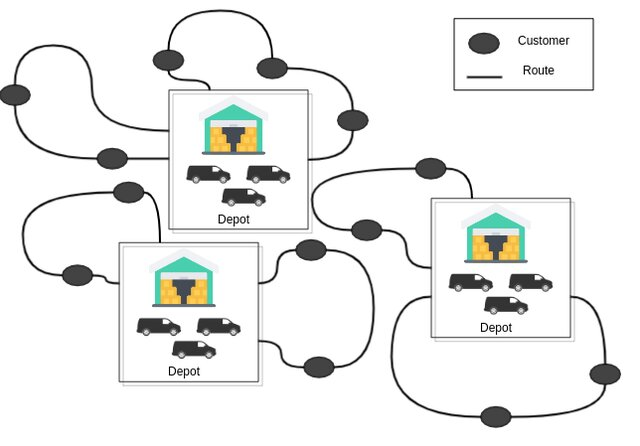
\includegraphics[width=0.8\textwidth]{fig/1.jpg}
	\caption{MDVRP图示}
	\label{fig:1}
\end{figure}

	
\section{相关工作}
本节回顾了多仓库车辆路径问题(MDVRP)、演化算法(EA)以及协同进化算法的现有研究。许多研究使用启发式和元启发式方法解决MDVRP,但像GCCA这样的协同方法在克服传统方法的可扩展性问题上显示出了优势。
	
\subsection{多仓库车辆路径问题(MDVRP)及其复杂性}

多仓库车辆路径问题(Multi-Depot Vehicle Routing Problem, MDVRP)是容量限制车辆路径问题(CVRP)的重要扩展,涉及多个仓库的协同调度和复杂约束下的路径规划。在MDVRP中,多个仓库作为配送起点和终点,车辆需满足容量限制和时间窗要求,同时完成对客户的需求分配 \cite{laporte1987exact, cordeau1997savings}。由于需要综合考虑仓库位置、车辆负载和服务时间窗,MDVRP相较于单仓库CVRP在复杂性和求解难度上均显著增加。

MDVRP的复杂性主要源于以下因素:首先,车辆容量和时间窗的约束限制了路径规划的可行性,大幅增加了搜索空间和计算复杂度 \cite{golden1998impact}。其次,仓库的多样性和地理位置分布需要同时考虑仓库与客户的分配策略,导致多仓库的全局调度优化更为复杂 \cite{salhi1991multi}. 多仓库路径优化属于NP难问题,难以通过传统的精确算法有效求解 \cite{clarke1964savings}。Laporte和Nobert提出的分支定界法 \cite{laporte1987exact} 尽管在小规模问题中能够找到最优解,但计算复杂度较高,不适用于大规模实例。Cordeau等人 \cite{cordeau1997savings} 提出的启发式节约算法和 Clarke 和 Wright 的分组分配法 \cite{clarke1964savings} 虽然能够提供较快的近似解,但在应对多重约束的复杂场景时往往陷入局部最优。



\subsection{求解多仓库车辆路径问题的启发式与元启发式算法}

求解多仓库车辆路径问题(MDVRP)的方法中,启发式和元启发式算法因其计算效率和灵活性得到了广泛应用。

经典启发式算法包括节约算法(Savings Method)和扫描算法(Sweep Algorithm),前者通过路径合并节约成本,后者通过基于地理位置的客户分组优化配送路线 \cite{clarke1964savings}。然而,这类方法虽然在小规模问题中能快速生成近似解,但在应对多仓库、多约束场景的复杂性时易于陷入局部最优 \cite{salhi1991multi}。

元启发式算法提供了更强的全局搜索能力,以求获得更优的解决方案。经典的元启发式算法包括遗传算法(Genetic Algorithm, GA)、模拟退火(Simulated Annealing, SA)和粒子群优化(Particle Swarm Optimization, PSO)。Golden等人 \cite{golden1998impact} 的研究表明,遗传算法在解决VRP时通过模拟自然选择和变异操作提升了算法的全局搜索性能,适合处理复杂的多仓库场景。Simulated Annealing利用随机扰动与温度下降机制避免局部最优,适用于路径复杂的MDVRP问题 \cite{cordeau1997savings}。粒子群优化算法则通过群体协作提升了解的多样性,在MDVRP求解中表现出较好的适应性 \cite{ai2009particle}。

尽管元启发式算法在求解MDVRP方面具有显著优势,单一方法难以兼顾求解速度与精度。近年来,许多研究探索了混合方法,以充分发挥各类算法的优势。Reimann等人 \cite{reimann2004heuristic} 的工作通过结合蚁群算法(Ant Colony Optimization, ACO)和节约算法提高了求解质量。Venkatesh和Singh (2015) 提出的遗传-模拟退火混合算法将遗传算法的全局搜索与模拟退火的局部搜索相结合,有效提升了解的质量与搜索速度 \cite{venkatesh2015hybrid}。这些混合方法为协同进化算法的引入奠定了基础,后者通过保持子群体的多样性进一步提升了求解效果,适应了MDVRP的高维搜索空间需求。

\subsection{优化问题中的合作协同进化算法}

合作协同进化算法(Cooperative Co-Evolution Algorithm,CCEAs)是一种基于生物进化的计算方法,尤其适用于复杂优化问题 \cite{potter1994cooperative, holland1992adaptation}。不同种群通过相互协作和竞争,维持解的多样性,从而增强了搜索的全局性和适应性,使得协同进化算法在具有较大搜索空间的多仓库车辆路径问题(MDVRP)中具有显著的潜力。

合作协同进化算法在复杂优化问题中的应用,已被证明能够有效提升求解质量和收敛速度。Holland (1992) 提出的遗传算法与协同进化思想结合的方法通过多样性维持机制避免了早熟收敛,提升了解的全局最优性 \cite{holland1992adaptation}。Potter和De Jong (1994) 的研究提出了协作协同进化(Cooperative Coevolution),通过将整体问题分解为子问题并使用独立种群解决各个子问题,从而增强算法的适应性和收敛性 \cite{potter1994cooperative}。

在物流与路径规划领域,协同进化算法表现出较高的求解效果。De Jong等人(2001)在动态环境中的路径规划问题中应用协同进化算法,通过种群间的协同进化,增强了算法对动态变化的适应能力 \cite{dejong2001evolutionary}。刘等人(2006)研究了基于协同进化的车辆路径规划方法,将车辆路径问题分解为多种群协作求解,显著提高了求解精度和搜索效率 \cite{liu2006vehicle}。这些研究验证了协同进化算法在路径规划问题中的有效性和实用性,为本文研究的基于协同进化的多仓库车辆路径优化方法奠定了理论基础。


\subsection{路径与调度中的禁忌搜索}

禁忌搜索(Tabu Search)是一种经典的局部优化算法,因其避免局部最优的特性而在路径优化和调度问题中表现优异。禁忌搜索通过维护一个“禁忌表”记录近期已访问的解状态,防止算法回到先前的解,从而跳出局部最优 \cite{glover1986future}。这种特性使得禁忌搜索在处理路径规划和车辆路径问题(VRP)中的局部最优陷阱时具有显著优势。Rego和Alidaee(1996)的研究中将禁忌搜索用于动态路径问题,通过限制解的退回与探索新路径的机制,在多约束的场景中取得了出色的优化效果 \cite{rego1996tabu}。Cordeau等人(1997)提出了一种基于禁忌搜索的VRP求解方法,通过结合禁忌搜索与启发式策略,实现了复杂路径规划的有效优化 \cite{cordeau1997savings}。

禁忌搜索与其他优化算法的结合已被证明可显著提升整体求解效果。Brandão(2004)通过将禁忌搜索与遗传算法结合应用于路径规划,显著提高了算法的收敛速度与求解质量 \cite{brandao2004tabu}。在MDVRP的高维搜索空间中,禁忌搜索的自适应搜索机制具有潜力。与协同进化框架相结合,禁忌搜索可以在保持解的多样性的同时有效探索高质量解,为复杂的多仓库路径规划提供了更具稳定性的解决方案。


\section{多仓库车辆路径问题描述}

多仓库车辆路径问题(Multi-Depot Vehicle Routing Problem, MDVRP)可以描述为在一个多重图 $G = (C, D, E)$ 上进行优化,其中:
\begin{itemize}
	\item $C$ 表示客户节点集合,共有 $N$ 个客户。
	\item $D$ 表示仓库节点集合,共有 $D$ 个仓库。
	\item $E$ 表示连接节点之间的弧集合。
\end{itemize}

设 $C = \{1, 2, \ldots, N\}$,$D = \{1, 2, \ldots, M\}$,$V = C \cup D$ 为所有节点的集合。弧集 $E = \{(i, j) | i, j \in V\} \setminus \{(i, j) | i, j \in D\}$,表示客户和仓库之间的连接关系。设第 $i$ 个客户的需求量为 $q_i$,节点 $i$ 和节点 $j$ 之间的距离为 $c_{ij}$。

系统中包含 $L$ 辆车,车辆集合为 $K = \{k_1, k_2, \ldots, k_L\}$。每辆车 $k$ 的最大容量为 $Q_k$,并且每个仓库 $d \in D$ 分配有一定数量的车辆,记为 $K(d)$。设 $K_d$ 表示仓库 $d$ 的最大车辆数量,$C(d)$ 表示分配给仓库 $d$ 的客户集合。

每辆车从一个仓库出发,在服务完分配的所有客户后返回该仓库。目标是确定每条路线的最优配送顺序,使得总行驶距离最小化,同时满足车辆容量的限制条件。

\subsection{决策变量}
\begin{align*}
	x_{ijk} &= 
	\begin{cases}
		1, & \text{若点 } i \text{ 在路径 } k \text{ 中直接位于点 } j \text{ 之前}; \\
		0, & \text{否则}.
	\end{cases} \\
	y_{kd} &= 
	\begin{cases}
		1, & \text{若车辆 } k \text{ 分配给仓库 } d; \\
		0, & \text{否则}.
	\end{cases}
\end{align*}

\subsection{优化模型}
目标函数:
\begin{equation}
	Z = \min \sum_{d \in D} \sum_{k \in K(d)} \sum_{i \in C(d) \cup \{d\}} \sum_{j \in C(d) \cup \{d\}} c_{ij} x_{ijk}
\end{equation}

约束条件:
\begin{align}
	&\sum_{k \in K} \sum_{j \in C} x_{djk} \leq K_d, \quad \forall d \in D \\
	&\sum_{d \in D} K_d \leq L \\
	&\sum_{d \in D} y_{kd} = 1, \quad \forall k \in K \\
	&\sum_{k \in K} \sum_{j \in C} x_{ijk} = 1, \quad \forall i \in C \\
	&\sum_{i \in C \backslash \{p\}} x_{ipk} = \sum_{j \in C \backslash \{p\}} x_{pjk}, \quad \forall p \in C, \forall k \in K \\
	&\sum_{j \in V} x_{ijk} \leq Q_k, \quad \forall k \in K \\
	&\sum_{j \in C} x_{djk} y_{kd} = 1, \quad \forall k \in K, \forall d \in D \\
	&\sum_{i \in C} x_{ijk} = 1, \quad \forall k \in K, \forall d \in D
\end{align}

在上述模型中:
\begin{itemize}
	\item 目标函数(1)最小化所有车辆的总成本(总距离)。
	\item 约束条件(2)和(3)限制每个仓库的车辆数量不超过其最大容量。
	\item 约束条件(4)确保每辆车只分配到一个仓库。
	\item 约束条件(5)规定每个客户只能被分配给一辆车。
	\item 约束条件(6)保证路径的连续性,每条路径上的车不会被重复分配。
	\item 约束条件(7)是车辆容量约束。
	\item 约束条件(8)和(9)保证每条路径只由一辆车服务。
\end{itemize}
	
\section{多仓库车辆路径问题求解}
\subsection{演化算法(EA)}

演化算法(Evolutionary Algorithm, EA)通过选择、交叉、变异等操作,使种群不断进化,逐步逼近问题的最优解。

\begin{figure}[htbp]
	\centering
	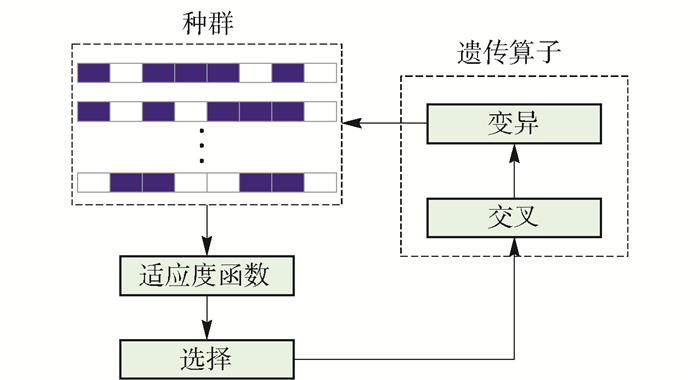
\includegraphics[width=0.8\textwidth]{fig/2.jpg}
	\caption{演化算法(EA)流程图}
	\label{fig:2}
\end{figure}

\subsubsection{编码}

在演化算法(EA)中,每个解(即个体)通过基因型编码(Genotype Encoding)来表示,该编码反映了车辆路径的具体信息。针对多仓库车辆路径问题(MDVRP)的复杂性和约束条件,采用分层编码方式以确保解的可行性和解码效率。首先,基因型编码用向量 $\bm{g} = (g_1, g_2, \ldots, g_n)$ 表示,其中每个元素 $g_i \in C \cup D$ 代表一个客户节点或仓库节点。基因型编码描述了客户和仓库在路径中的排列顺序,确保每个客户节点都唯一地分配至一个车辆路径。为了获得实际的路径规划方案,将基因型编码进一步解码为现象型(Phenotype Decoding),即具体的车辆路线。设现象型为向量 $\bm{p} = (p_1, p_2, \ldots, p_m)$,其中 $p_j$ 表示车辆执行的具体路径,满足车辆容量限制和路径连续性。解码后的现象型能够确保每辆车仅服务于其分配的客户群体,路径上所有客户节点的总需求量不超过车辆容量 $Q_k$,即 $\sum_{i \in C_j} q_i \leq Q_k$,其中 $C_j$ 表示车辆 $j$ 的服务客户集合。

\subsubsection{适应度函数}

适应度函数用于评估每个个体解的质量,其目标是最小化所有车辆的总行驶距离,同时满足多仓库车辆路径问题(MDVRP)的各类约束条件。适应度函数定义为:
\begin{equation}
	\text{Fitness} = \sum_{r \in \text{Routes}} \text{Distance}_r + P,
\end{equation}
其中,$\text{Distance}_r$ 表示车辆在路径 $r$ 上的总行驶距离,而 $P$ 为惩罚项,用于在违反容量或时间约束时加入额外的成本。具体而言,适应度函数需满足以下优化目标:首先,所有车辆的总行驶距离 $\sum_{r \in \text{Routes}} \text{Distance}_r$ 需最小化,以提高运输效率。其次,每个客户节点 $i \in C$ 必须由唯一的车辆服务,这通过以下约束条件来保证:
\begin{equation}
	\sum_{k \in K} x_{ijk} = 1, \quad \forall i \in C,
\end{equation}
其中,$x_{ijk}$ 是二元决策变量,若客户 $i$ 被分配到车辆 $k$ 的路径上,则 $x_{ijk} = 1$,否则 $x_{ijk} = 0$。最后,适应度函数还需确保每辆车的路径满足容量和时间限制,即每辆车 $k$ 的服务客户总需求不超过其容量 $Q_k$,表示为:
\begin{equation}
	\sum_{i \in C_k} q_i \leq Q_k, \quad \forall k \in K,
\end{equation}
其中 $C_k$ 为分配给车辆 $k$ 的客户集合,$q_i$ 为客户 $i$ 的需求量。

\subsection{演化操作符}

\paragraph{选择(Selection)} 

选择操作通过\textbf{锦标赛选择(Tournament Selection)}方法,从当前种群中筛选出适应度较高的个体,以加速算法向最优解的收敛。锦标赛选择随机从种群中挑选若干个体进行比较,并保留其中适应度最高的个体,从而在保证解的多样性的同时平衡全局搜索和局部开发能力。假设从种群中随机抽取了 $k$ 个体 $\{i_1, i_2, \ldots, i_k\}$,则选中的个体 $i^*$ 满足:
\[
i^* = \arg \max_{i \in \{i_1, i_2, \ldots, i_k\}} \text{Fitness}_i,
\]
其中 $\text{Fitness}_i$ 表示个体 $i$ 的适应度值。通过锦标赛选择,可以确保优质解在种群中得以延续,加速收敛的同时提升算法的探索能力。

\paragraph{交叉(Crossover)}

交叉操作采用\textbf{部分映射交叉(Partially Mapped Crossover, PMX)}方法,以生成新的子代个体,增强种群多样性并加速局部搜索。PMX方法在两个父代个体 $p_1$ 和 $p_2$ 中随机选择一个子序列,将该子序列直接映射到子代中,以确保子代继承该子序列的基因信息。设交叉子序列的范围为 $[s, t]$,则生成的子代个体 $c$ 的基因序列可表示为:
\[
c[i] = \begin{cases} 
	p_1[i], & \text{若 } i \in [s, t], \\
	\text{map}(p_2[i]), & \text{否则},
\end{cases}
\]
其中 $i \in [1, n]$,$\text{map}(\cdot)$ 表示位置映射操作。在确保基因信息有序的前提下,PMX操作有效扩展了算法的搜索空间,并在种群中引入更高的多样性。

\paragraph{变异(Mutation)}

变异操作使用\textbf{交换变异(Swap Mutation)}方法,通过引入随机性来增强解的多样性,从而避免种群陷入局部最优。交换变异在个体的路径中随机选择两个客户节点并交换其位置,从而改变路径结构。具体而言,对于路径 $\bm{p}$ 中的两个位置 $i$ 和 $j$,交换变异定义为:
\[
\bm{p}' = \text{swap}(p_i, p_j), \quad i, j \in \{1, \ldots, n\}, \quad i \neq j,
\]
其中 $p_i$ 和 $p_j$ 分别表示路径 $\bm{p}$ 中的两个客户节点。交换变异在不破坏现有路径结构的情况下引入新的解,确保种群在搜索空间中有更广泛的探索。

	
\subsection{贪婪协同进化算法(GCEA)}

贪婪协同进化算法(Greedy Cooperative Co-Evolutionary Algorithm, GCEA)通过将多仓库车辆路径问题(MDVRP)分解为多个子问题并协同求解,以有效应对其复杂性。首先,将总体种群 $P$ 划分为 $m$ 个子种群 $\{P_1, P_2, \ldots, P_m\}$,每个子种群 $P_i$ 对应一个独立的子问题。子问题划分时确保每个子种群的客户节点分布相对均衡,并满足车辆容量及路径长度约束。

\begin{figure}[htbp]
	\centering
	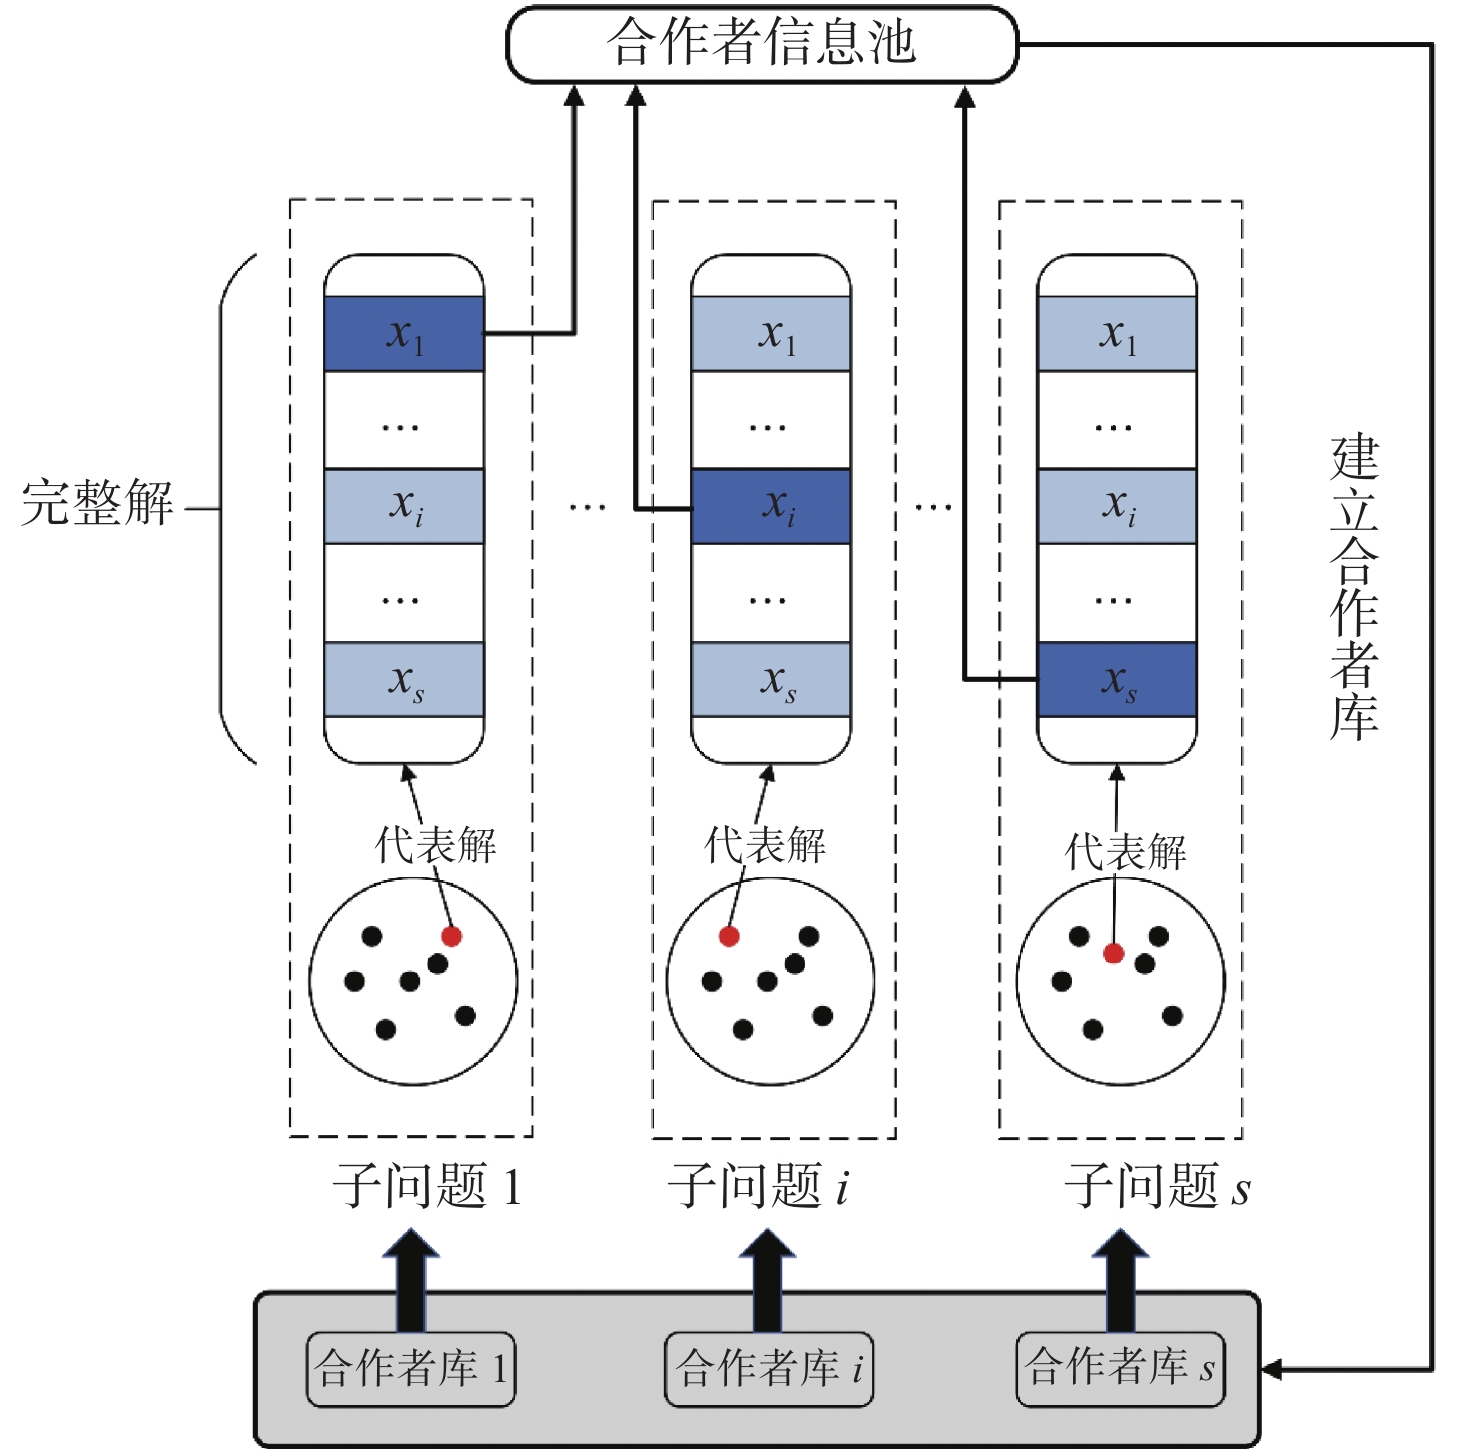
\includegraphics[width=0.6\textwidth]{fig/3.jpg}
	\caption{贪婪协同进化算法(GCEA)流程图}
	\label{fig:3}
\end{figure}

在子种群进化中,采用贪婪算法对每个子种群 $P_i$ 进行局部优化,逐步选择对路径优化贡献最大的客户节点,构建最优路径。为增加解的多样性和全局搜索能力,子种群间定期进行解的交换。各子种群独立进化完成后,GCEA通过合并各子种群的解构成全局解。合并过程将各子问题中的路径进行组合,并调整相邻子种群的边界,确保全局解 $\bm{P}$ 的连续性及所有约束的满足。设各子种群的解分别为 $\bm{p}_1, \bm{p}_2, \ldots, \bm{p}_m$,则全局解 $\bm{P}$ 表示为:
\[
\bm{P} = \bigcup_{i=1}^{m} \bm{p}_i,
\]
其中 $\bm{P}$ 满足所有多仓库车辆路径问题的约束条件。通过分布式优化和结果合并,GCEA能够有效提升MDVRP的求解效率和解的质量。

\subsection{禁忌搜索优化的贪婪协同进化算法(TGCEA)}

禁忌搜索优化的贪婪协同进化算法(Tabu-Greedy Cooperative Evolutionary Algorithm, TGCEA)通过在局部搜索中引入禁忌机制来避免陷入局部最优,从而提升了搜索过程的多样性和全局最优解的可达性。

\subsubsection{禁忌搜索机制}

禁忌搜索(Tabu Search)通过引入禁忌表(Tabu List)机制,有效防止在搜索过程中陷入循环与局部最优。禁忌表用于记录最近访问的解,避免算法短期内重新采纳已访问过的劣解,从而增强解的多样性。禁忌表的更新过程设定一个最大容量 $\tau$,当禁忌表达到容量上限时,将最早进入的解移出,确保表的动态维护。

在生成候选解时,若新解 $s_{\text{new}}$ 已在禁忌表中,则对其适应度值进行惩罚修正,以降低其被再次选中的概率。设 $s_{\text{new}}$ 的原始适应度值为 $\text{Fitness}(s_{\text{new}})$,若 $s_{\text{new}} \in \text{Tabu List}$,则通过以下公式进行适应度修正:
\[
\text{Fitness}'(s_{\text{new}}) = \text{Fitness}(s_{\text{new}}) + \lambda P,
\]
其中 $\lambda$ 为惩罚系数,$P$ 为固定惩罚值。此修正增加了禁忌解的适应度值,使得其在后续选择中被采纳的概率显著降低,有效提升了解的全局搜索能力。



\subsubsection{禁忌搜索与贪婪优化的结合}

首先,对当前解 $s$ 通过变异和交叉操作生成一组候选解 $\{s_{\text{new},1}, s_{\text{new},2}, \ldots, s_{\text{new},k}\}$。对于每个候选解 $s_{\text{new},i}$,若其在禁忌表中,则根据禁忌条件对其适应度施加惩罚,使其选择概率降低。随后,采用贪婪选择策略,从所有候选解中选择适应度最优的解作为新解,若该解满足禁忌条件且具有更优的适应度值,则更新当前解,并将该解加入禁忌表。

\subsubsection{TGCEA全局优化目标}

TGCEA旨在找到符合多仓库车辆路径问题(MDVRP)约束的全局最优解 $\bm{P}^*$,即:
\[
\bm{P}^* = \arg \min_{\bm{P}} \left( \sum_{r \in \text{Routes}} \text{Distance}_r + \sum_{\text{penalty}} P \right),
\]
其中 $\text{Distance}_r$ 表示路径 $r$ 的总行驶距离,$P$ 为因违反约束而引入的惩罚项。此优化目标确保在路径规划中总距离最小化,同时严格满足所有路径的容量和时间约束条件。

	
\section{实验配置}

\subsection{数据集描述}

本实验使用了两个不同的多仓库车辆路径问题(MDVRP)数据集,以测试算法在不同场景下的表现。数据集1较为简洁,包含12个节点,其中2个节点为仓库(ID: 11-12),10个节点为客户。该数据集的仓库节点容量为200,服务时间窗为[0, 1000],而客户节点的需求量在1到24之间不等,每个客户节点配有特定的时间窗。例如,客户节点1的需求量为12,其时间窗为[399, 525]。数据集2包含54个节点,包括4个仓库节点(ID: 51-54)和50个客户节点。仓库节点的容量设定为80单位,而客户节点的需求量则在5到41之间不等。这两个数据集分别具有不同的节点配置、需求量和约束条件,能够有效评估算法在不同规模和复杂度条件下的适应性和求解效率。

\subsection{实验环境与评价指标设置}

\subsubsection{实验环境}

\begin{itemize}
	\item \textbf{操作系统:} Linux系统
	\item \textbf{Python版本:} Python 3.11
	\item \textbf{CPU:} Intel Core i9-14900HX
	\item \textbf{GPU:} NVIDIA RTX 4090D
\end{itemize}

\subsubsection{评价指标}
为了全面评估算法的性能和稳定性,本实验从任务设置、试验次数、数据记录与可视化三个方面进行系统评价。首先,实验进行30次独立试验,记录每次试验的最优适应度值和运行时间,以评估算法在不同试验条件下的稳定性与执行效率。实验还详细记录每次试验的最优适应度值及其生成的迭代次数,并通过图表形式展示解的质量和计算效率,以便于全面分析算法的整体性能。此外,通过多项评价指标进一步量化算法表现,包括解的质量、计算效率以及鲁棒性和稳定性。解的质量指标用于衡量算法在解空间中找到高质量解的能力;计算效率通过运行时间来量化算法的时间复杂度和计算成本;鲁棒性和稳定性则基于多次试验结果的波动情况,评估算法在不同试验条件下的表现一致性,确保算法在高效求解的同时具备较高的可靠性。


	
\section{实验结果}
\textbf{数据集1(带时间窗的MDVRP):}

\begin{figure}[htbp]
	\centering
	\begin{subfigure}[b]{0.316\textwidth}
		\centering
		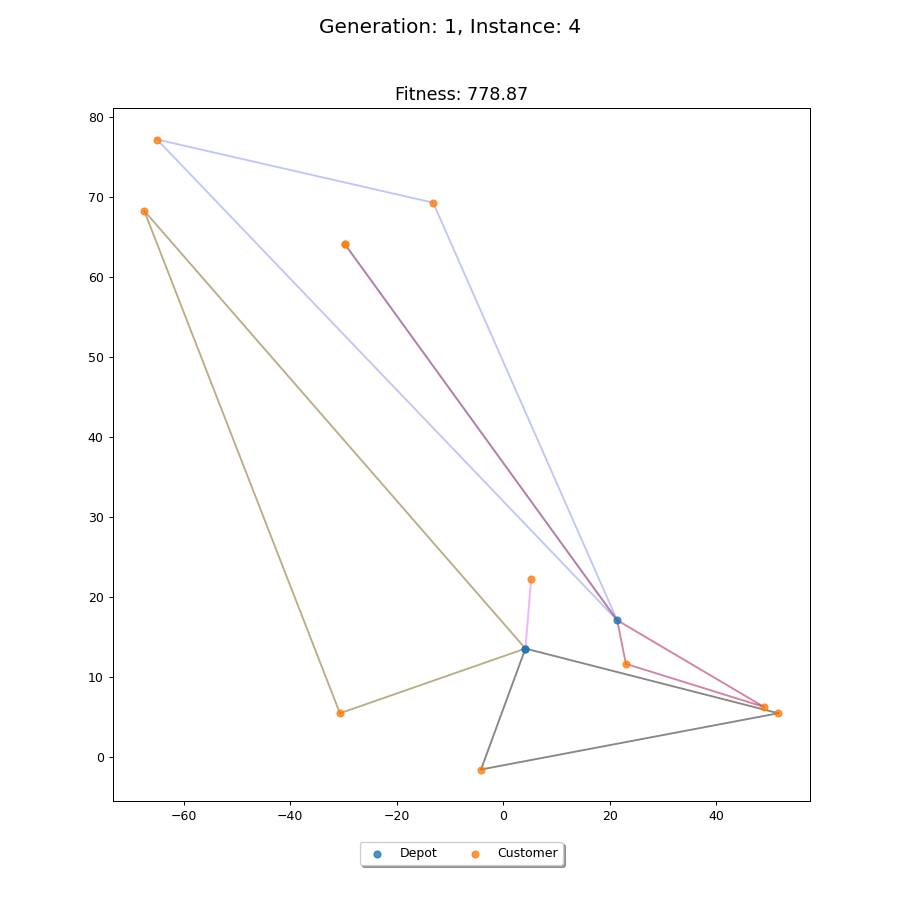
\includegraphics[width=\textwidth]{fig/5.png}
	\end{subfigure}
	\hspace{2pt} % Reduce horizontal space between images
	\begin{subfigure}[b]{0.4\textwidth}
		\centering
		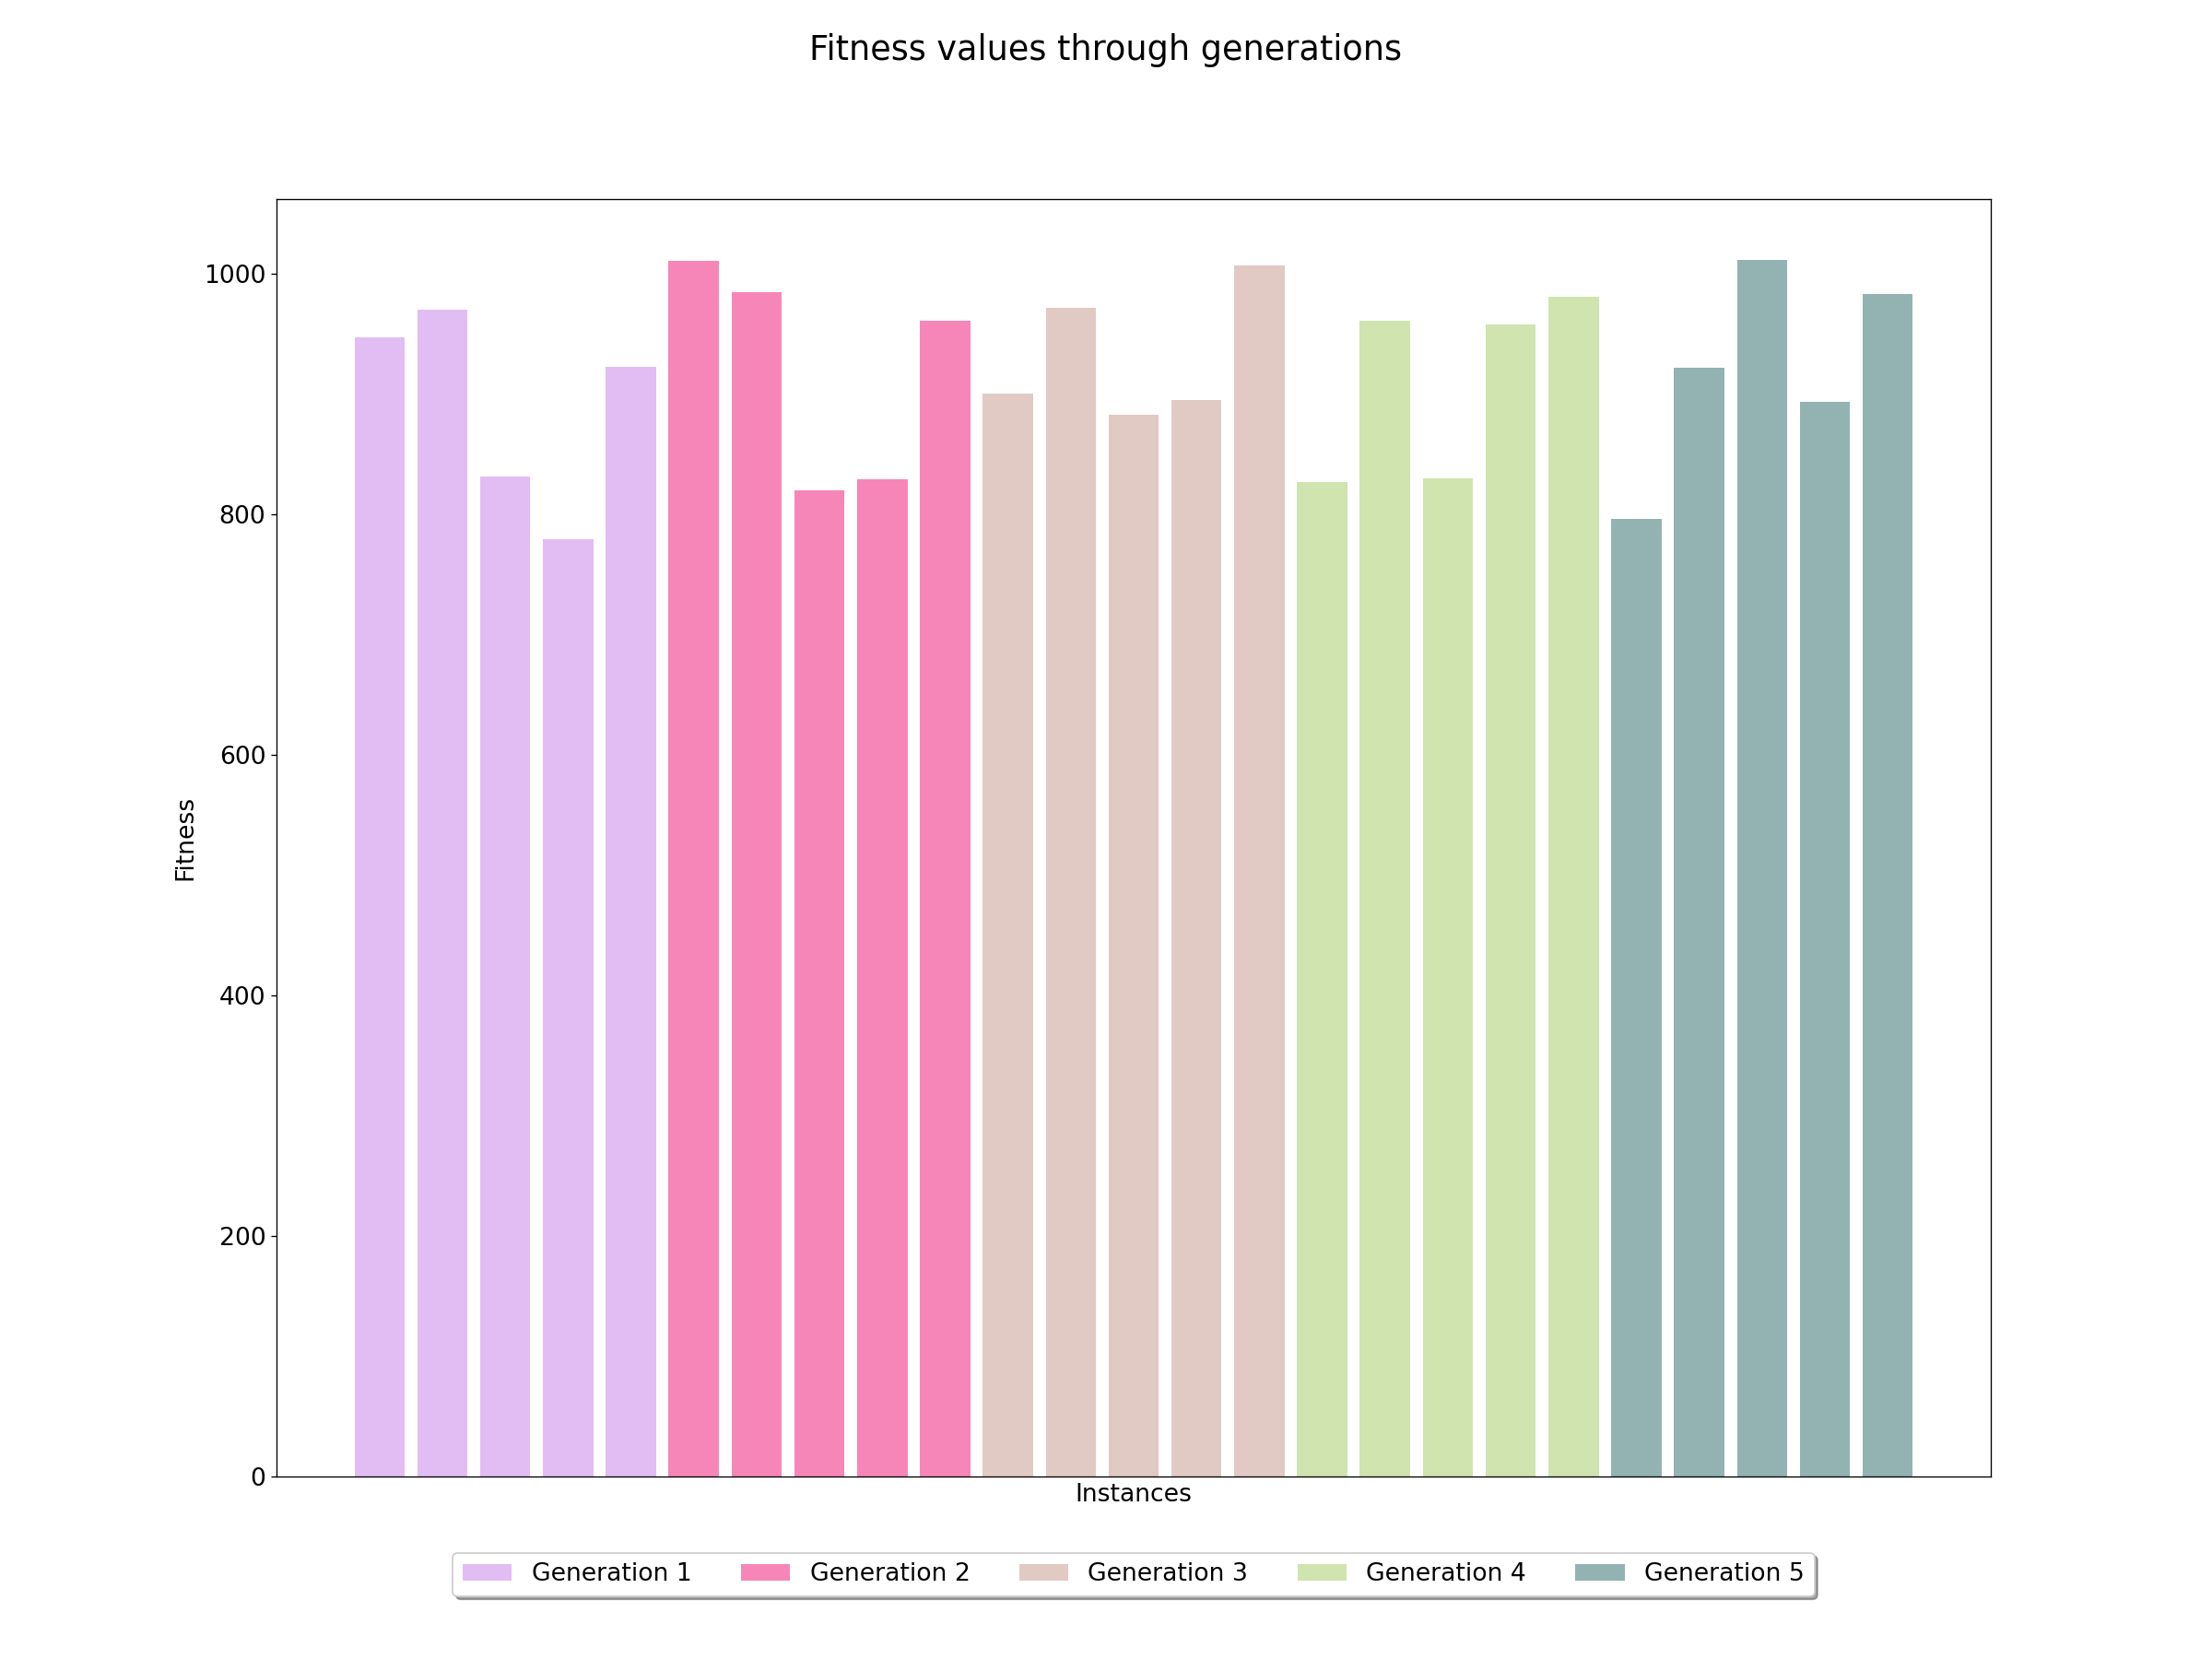
\includegraphics[width=\textwidth]{fig/6.png}
	\end{subfigure}
	\caption{进化算法最优各代的适应度值}
\end{figure}

\vspace{-12pt} % Reduce vertical space

\begin{figure}[htbp]
	\centering
	\begin{subfigure}[b]{0.316\textwidth}
		\centering
		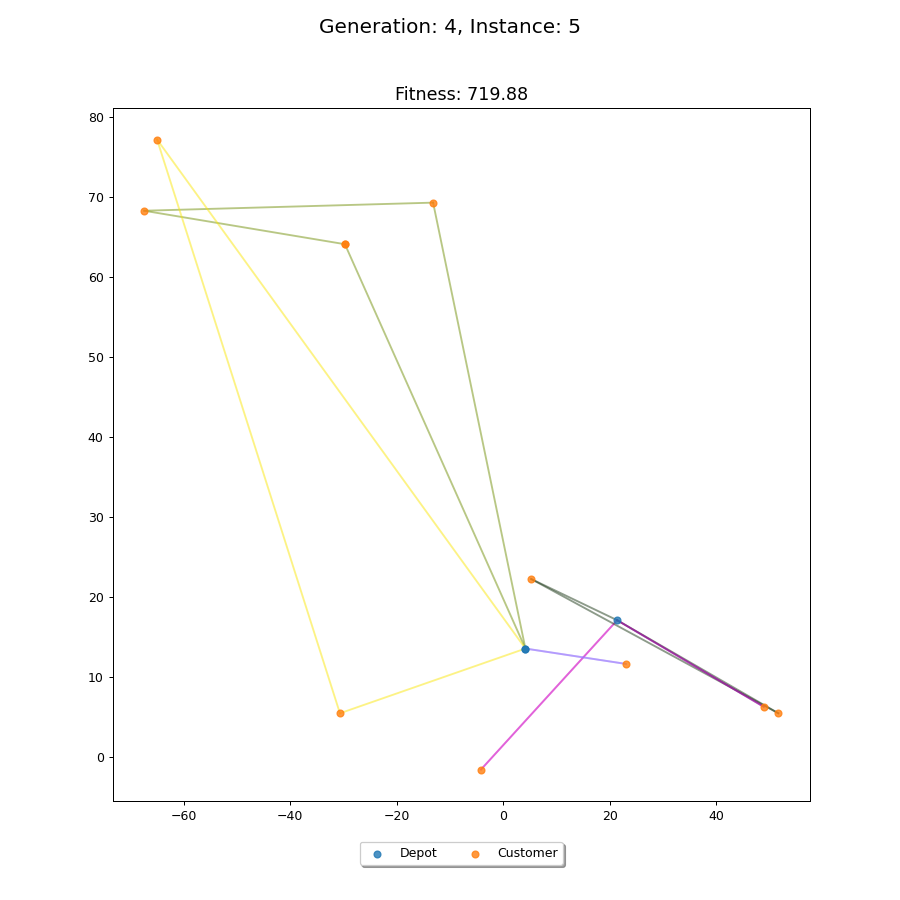
\includegraphics[width=\textwidth]{fig/7.png}
	\end{subfigure}
	\hspace{2pt} % Reduce horizontal space between images
	\begin{subfigure}[b]{0.4\textwidth}
		\centering
		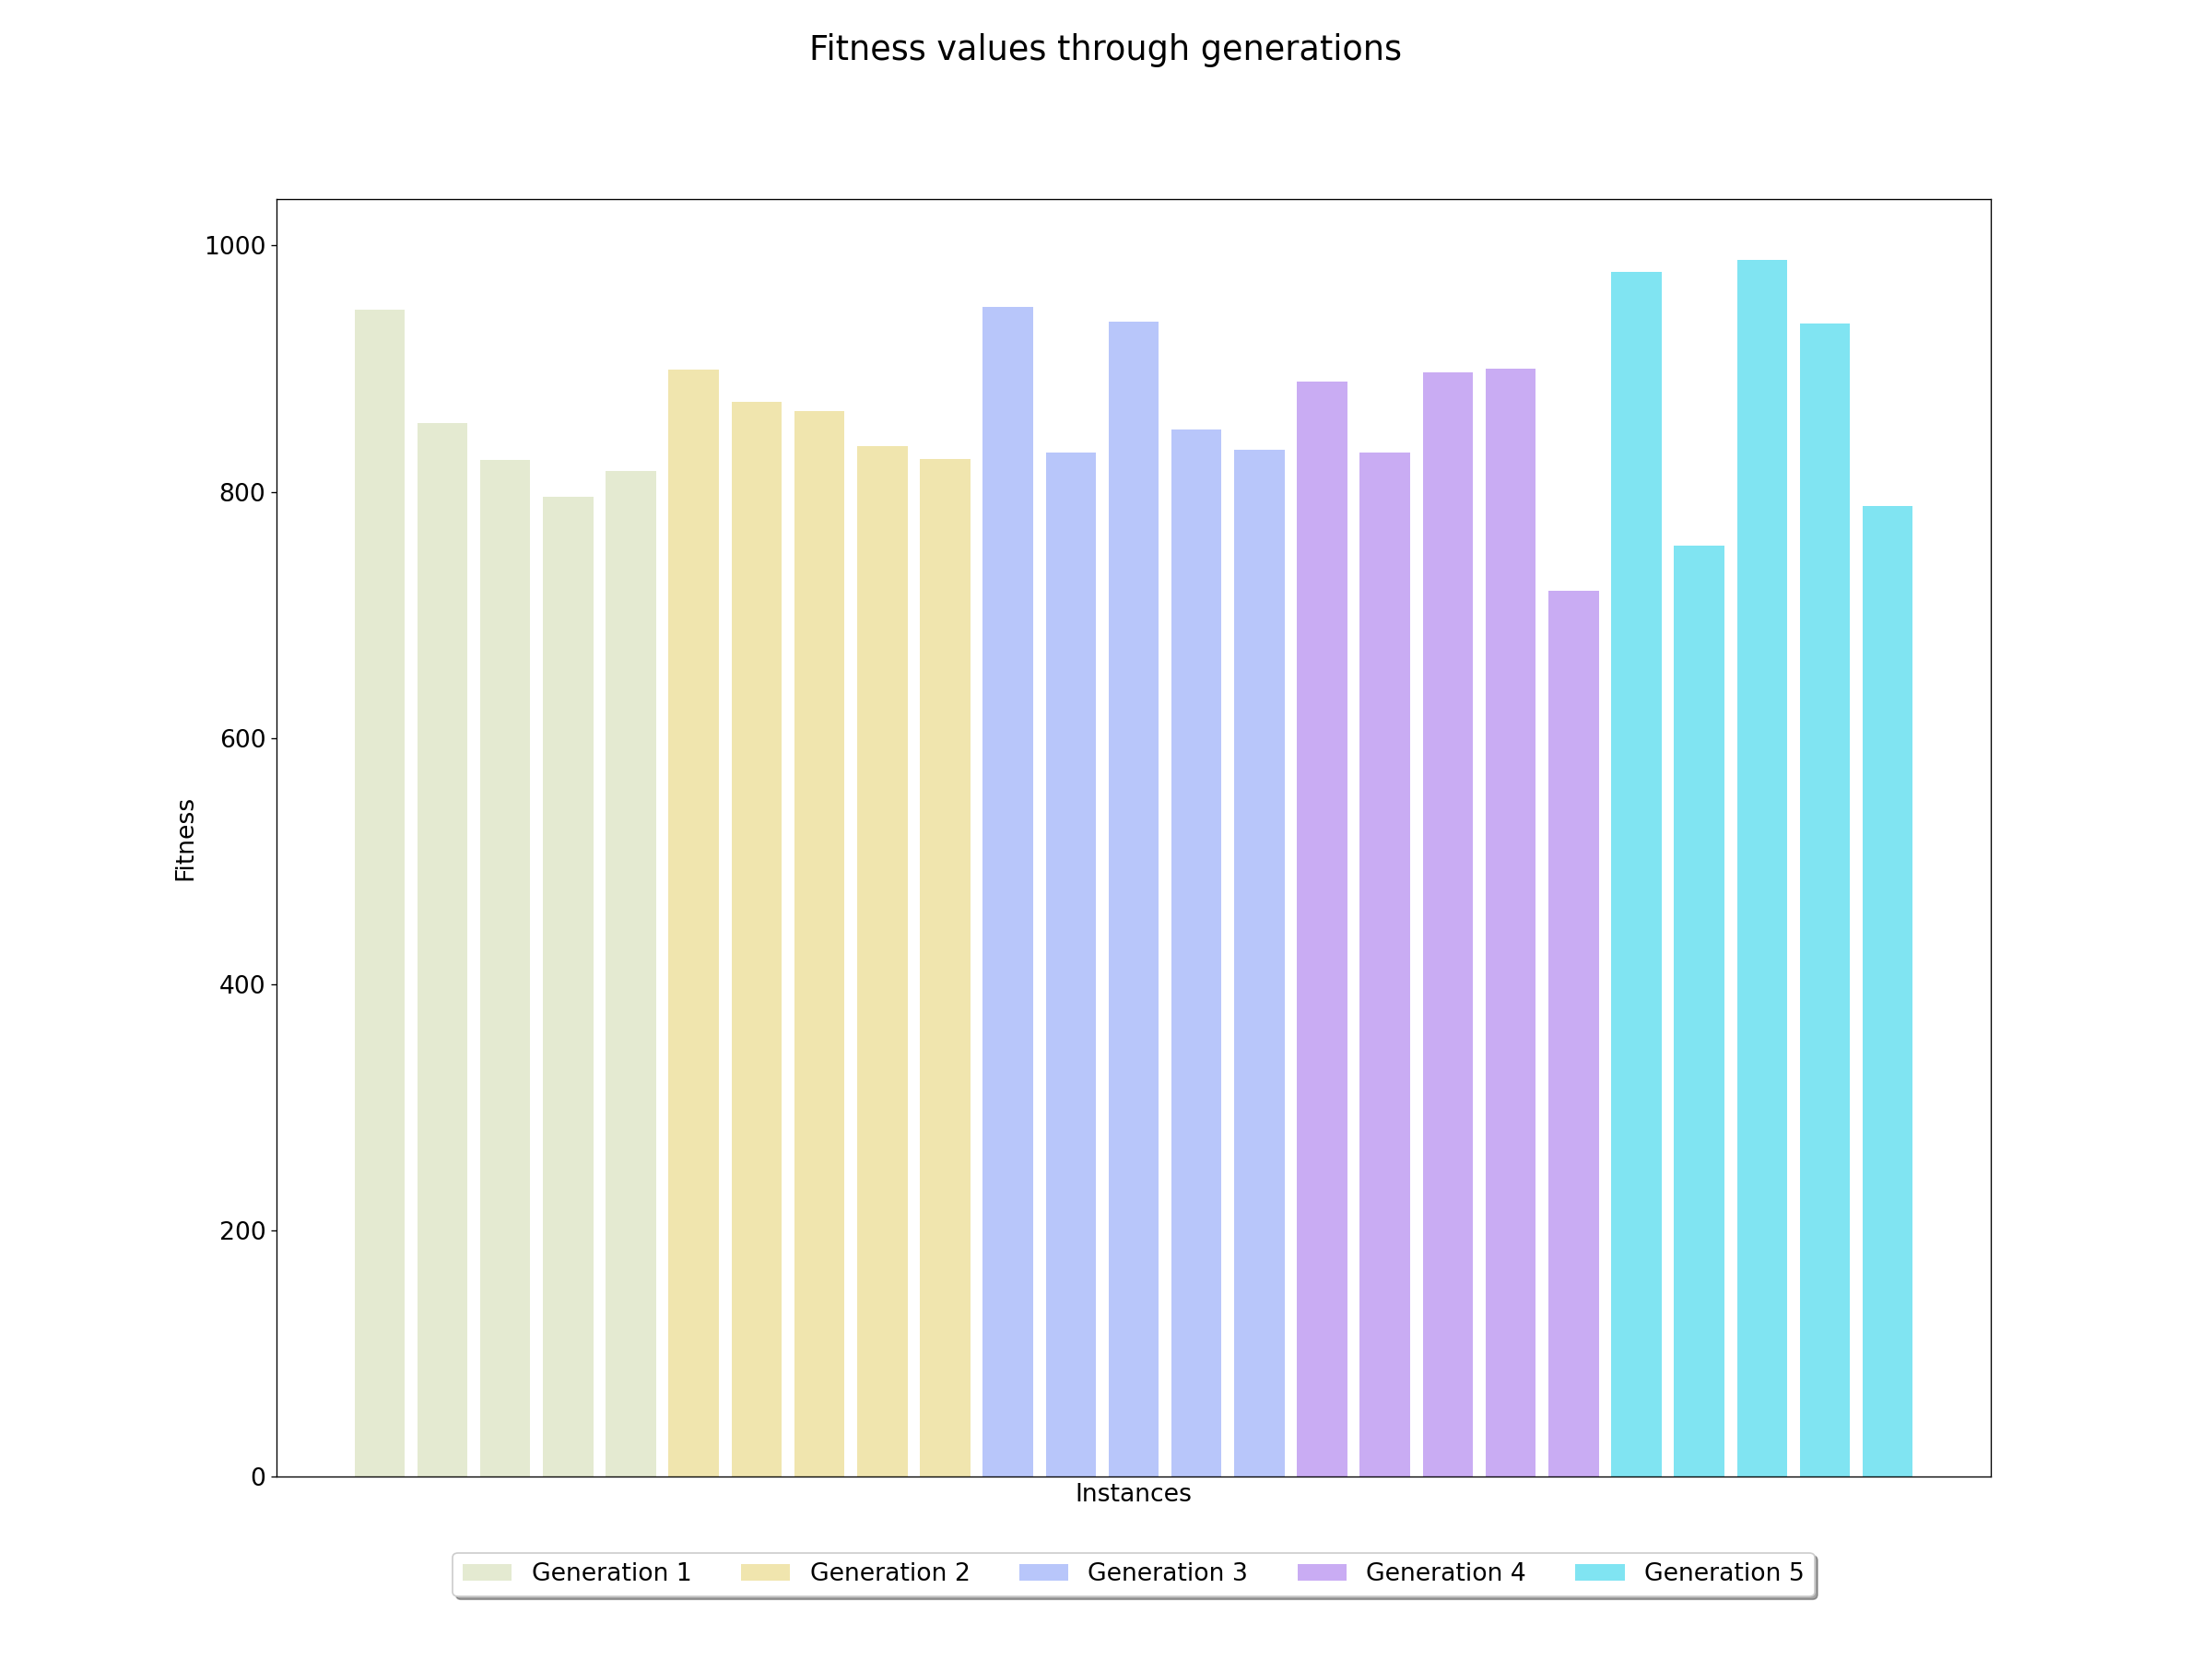
\includegraphics[width=\textwidth]{fig/8.png}
	\end{subfigure}
	\caption{贪婪协同进化算法最优各代的适应度值}
\end{figure}

\vspace{-12pt} % Reduce vertical space

\begin{figure}[htbp]
	\centering
	\begin{subfigure}[b]{0.316\textwidth}
		\centering
		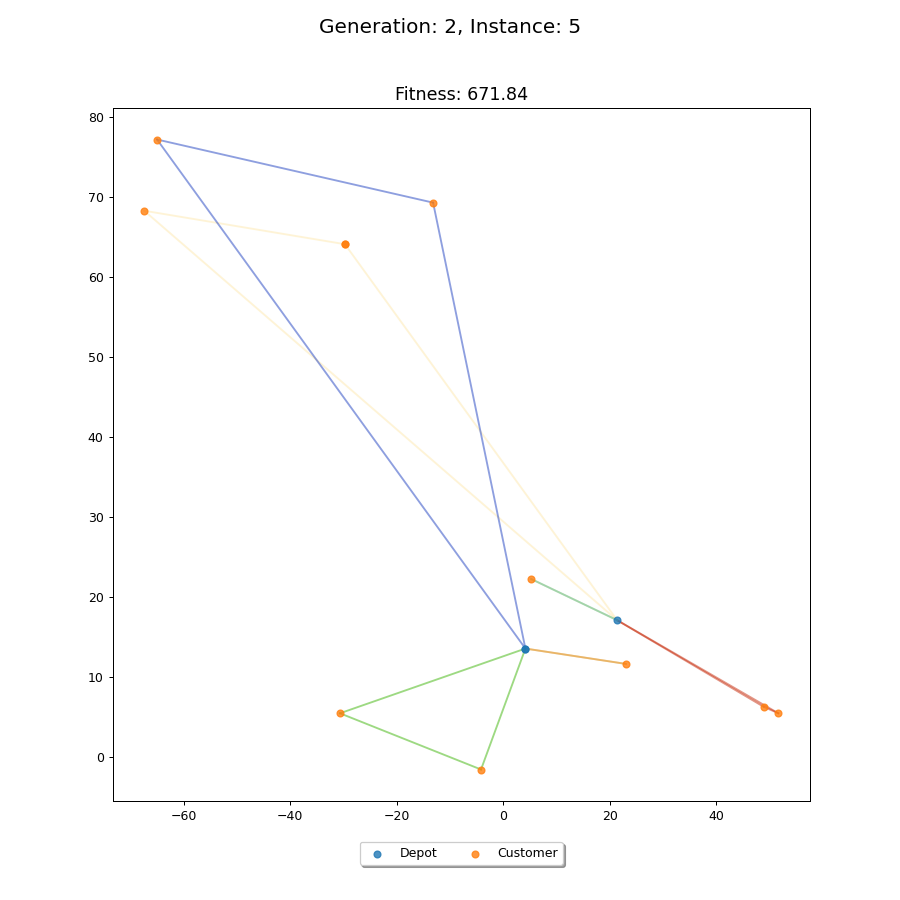
\includegraphics[width=\textwidth]{fig/9.png}
	\end{subfigure}
	\hspace{2pt} % Reduce horizontal space between images
	\begin{subfigure}[b]{0.4\textwidth}
		\centering
		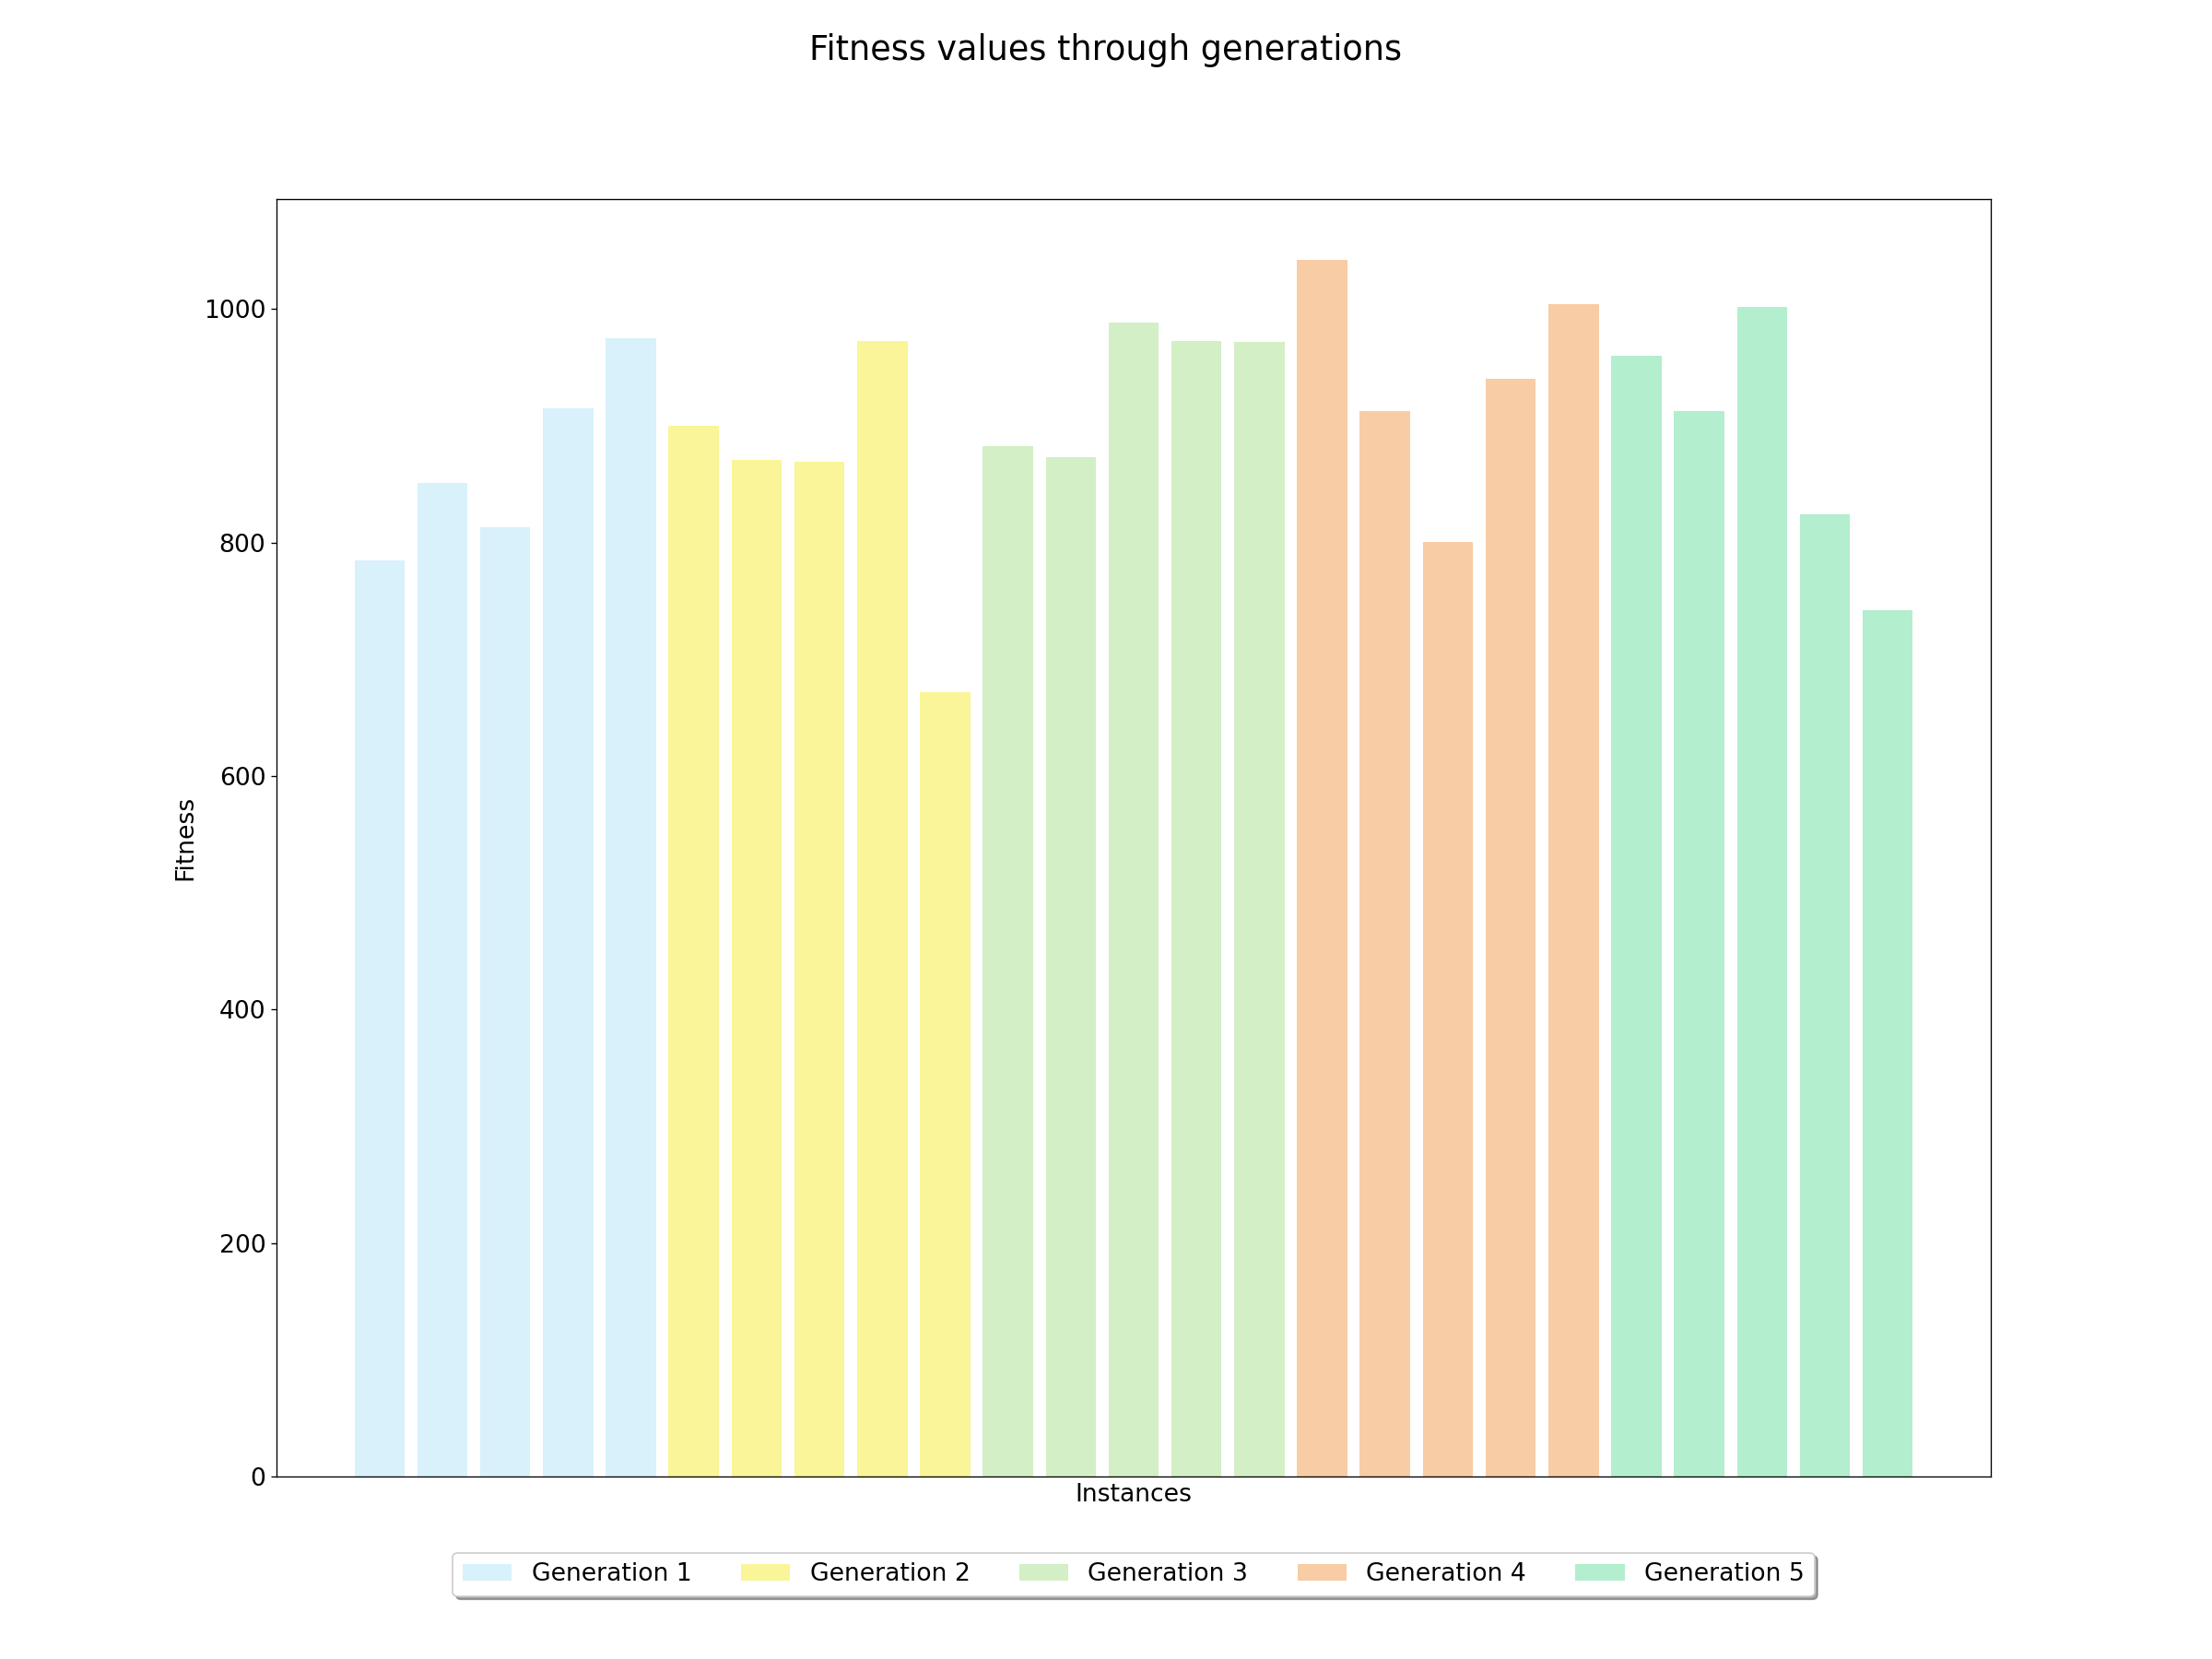
\includegraphics[width=\textwidth]{fig/10.png}
	\end{subfigure}
	\caption{禁忌搜索优化的贪婪协同进化算法最优各代的适应度值}
\end{figure}

\vspace{1em}
\noindent 因正文篇幅限制,所有求解结果请参见附录。

\newpage
\textbf{数据集2(不带时间窗的MDVRP):}

\begin{figure}[htbp]
	\centering
	\begin{subfigure}[b]{0.316\textwidth}
		\centering
		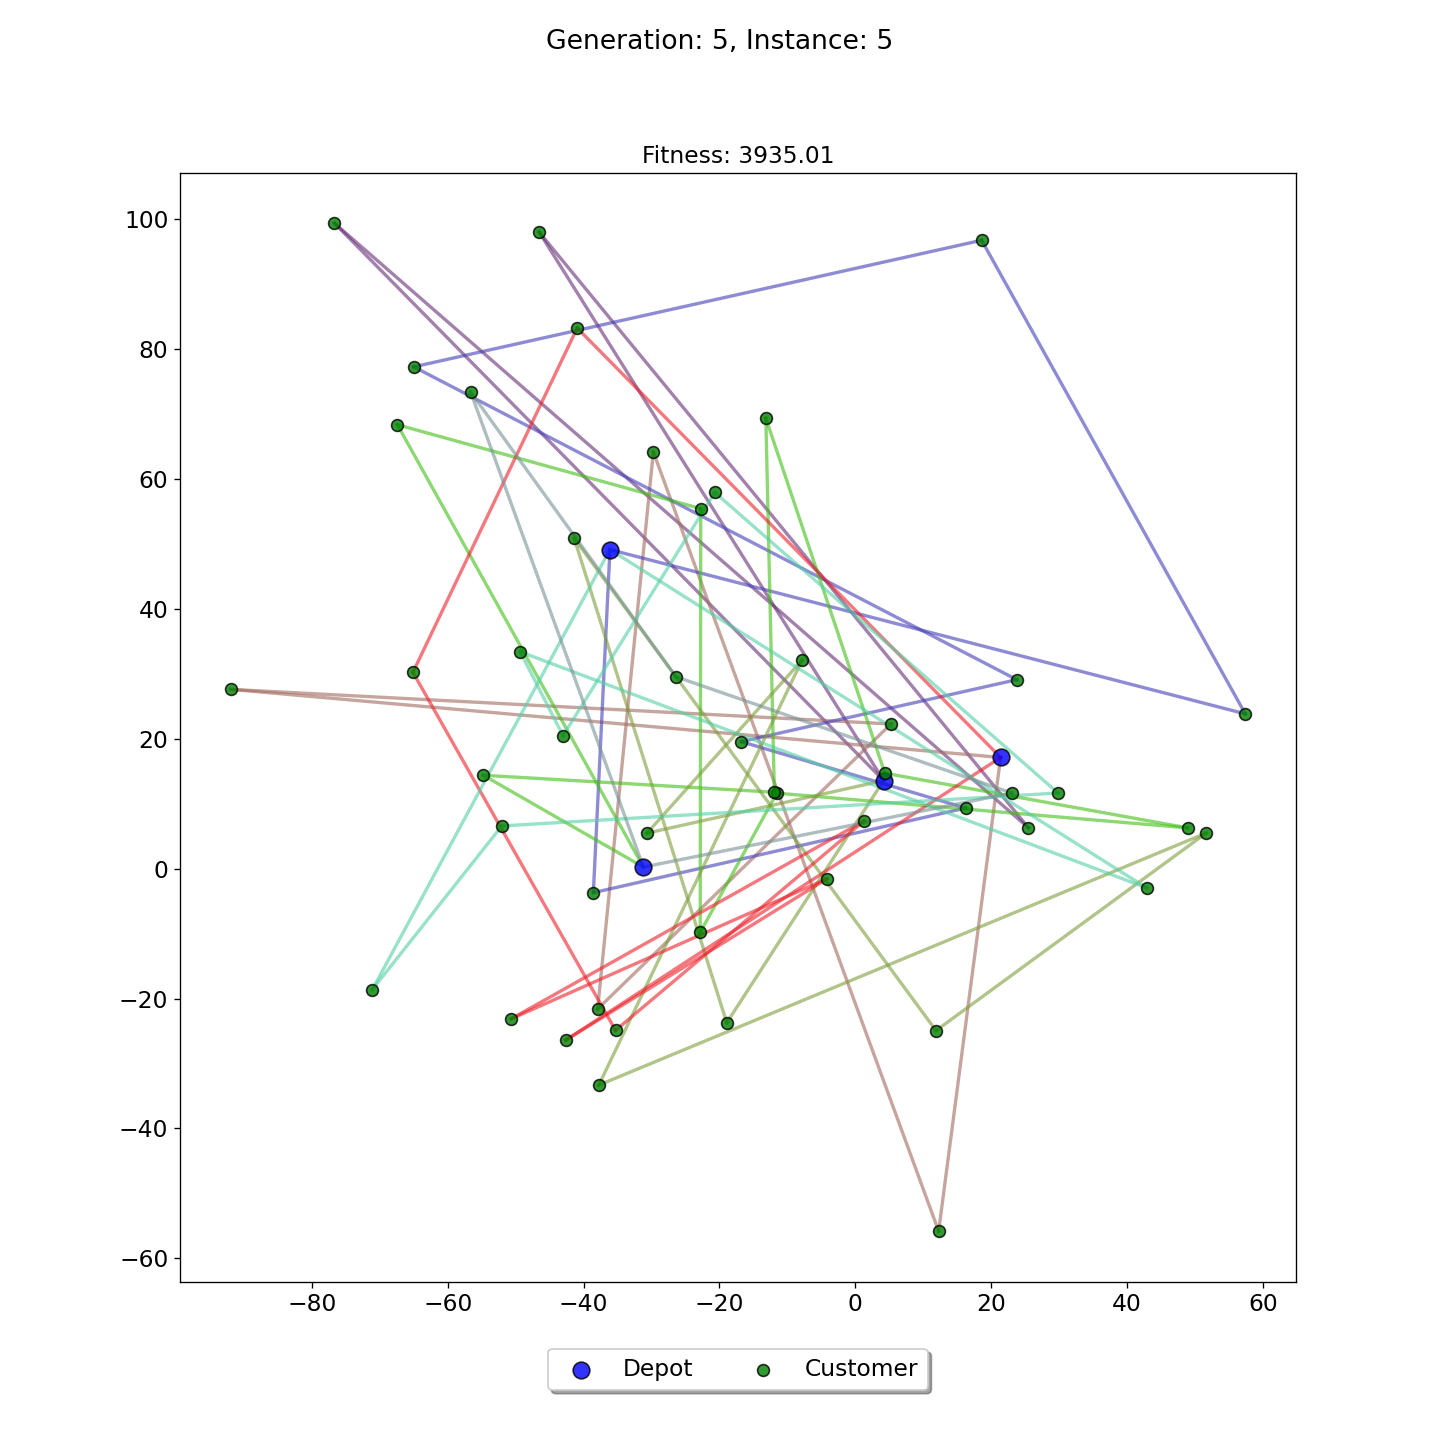
\includegraphics[width=\textwidth]{fig/11.png}
	\end{subfigure}
	\hspace{2pt} % Reduce horizontal space between images
	\begin{subfigure}[b]{0.4\textwidth}
		\centering
		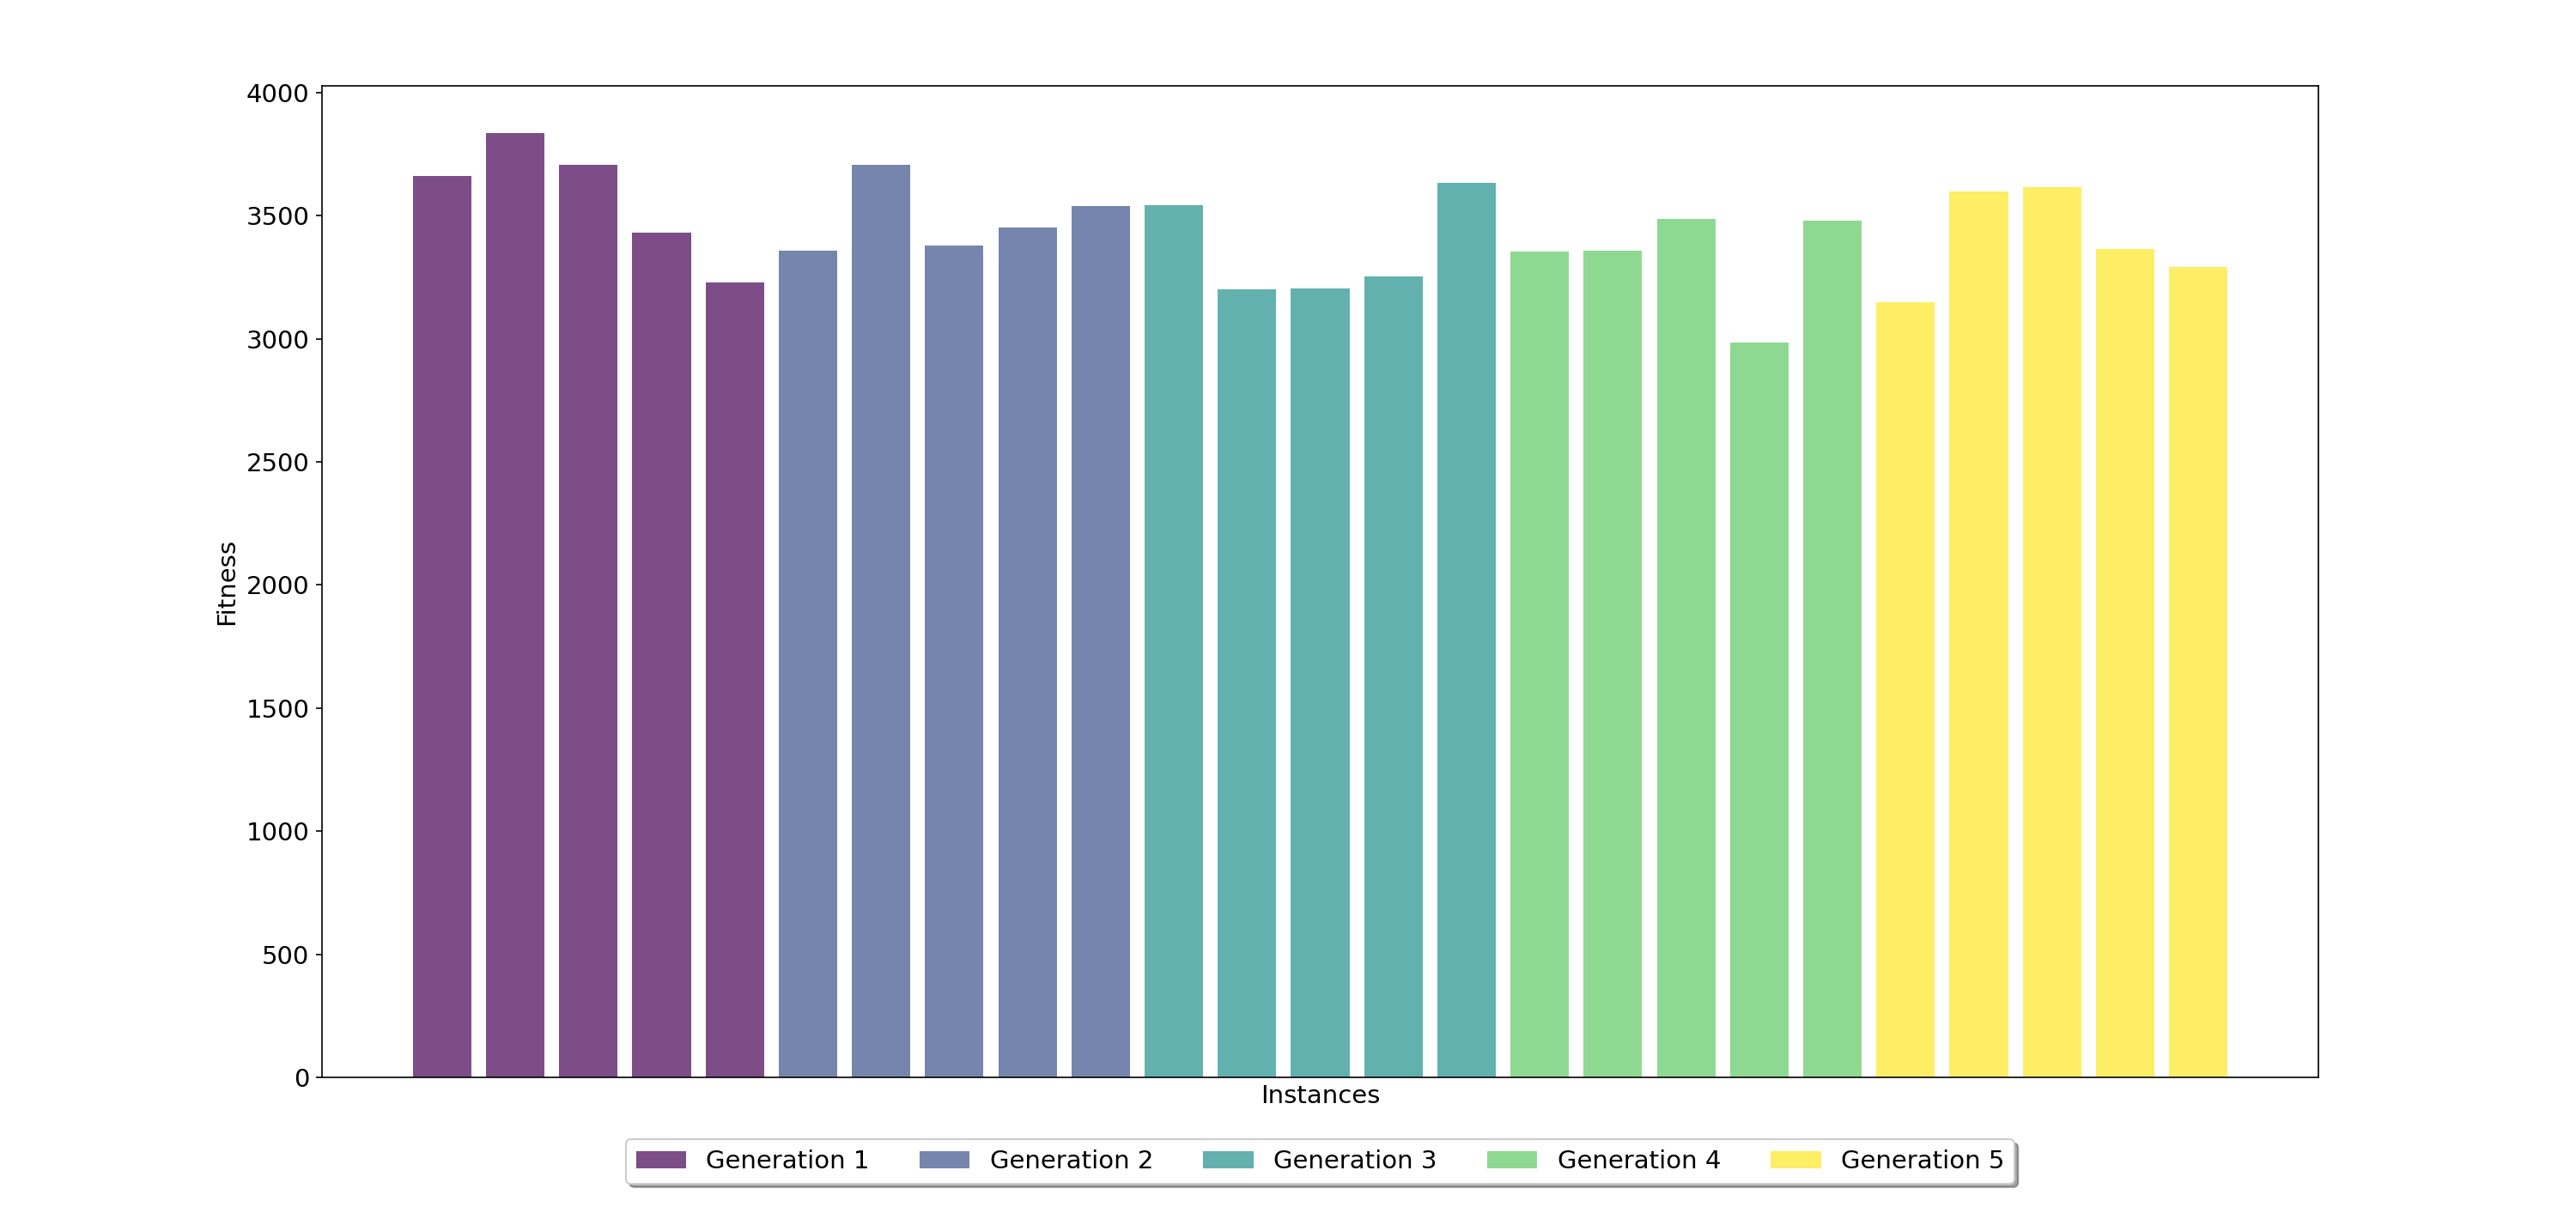
\includegraphics[width=\textwidth]{fig/12.png}
	\end{subfigure}
	\caption{进化算法最优各代的适应度值}
\end{figure}

\vspace{-12pt} % Reduce vertical space

\begin{figure}[htbp]
	\centering
	\begin{subfigure}[b]{0.316\textwidth}
		\centering
		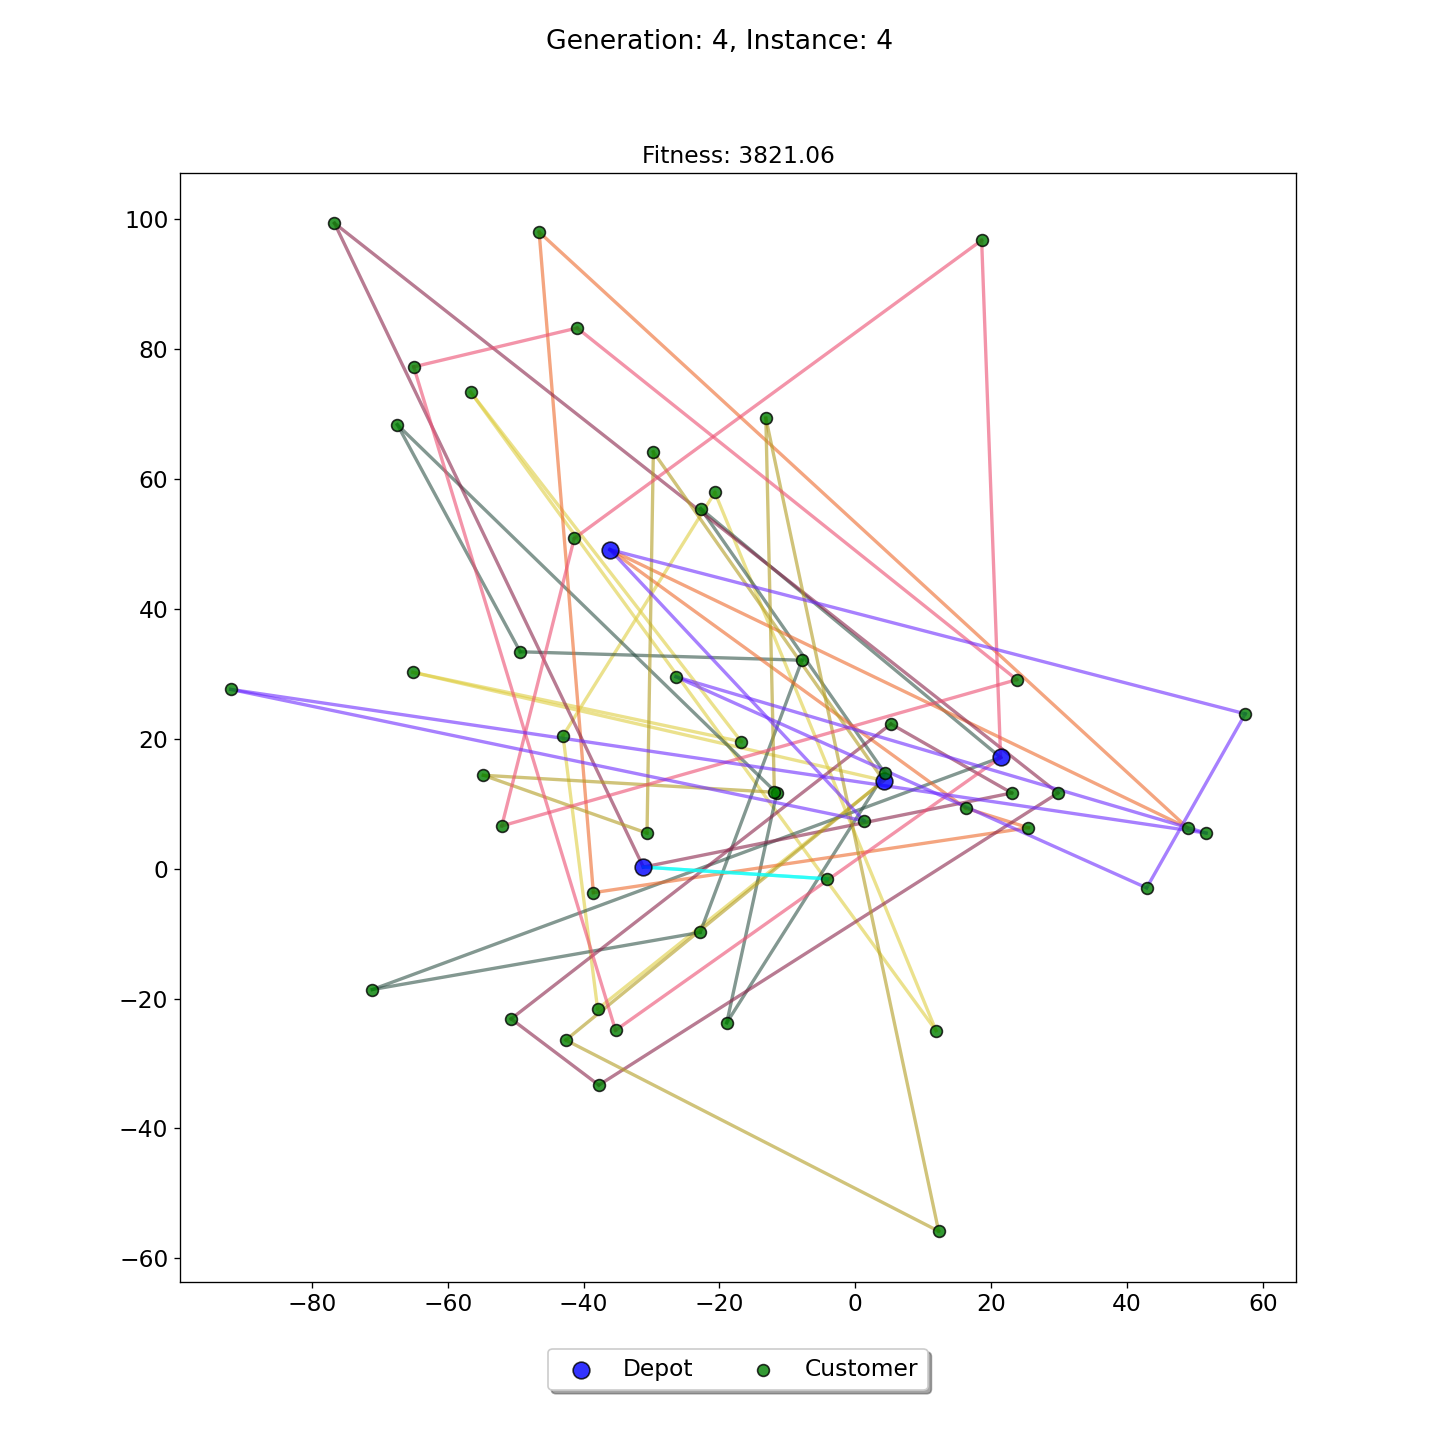
\includegraphics[width=\textwidth]{fig/13.png}
	\end{subfigure}
	\hspace{2pt} % Reduce horizontal space between images
	\begin{subfigure}[b]{0.4\textwidth}
		\centering
		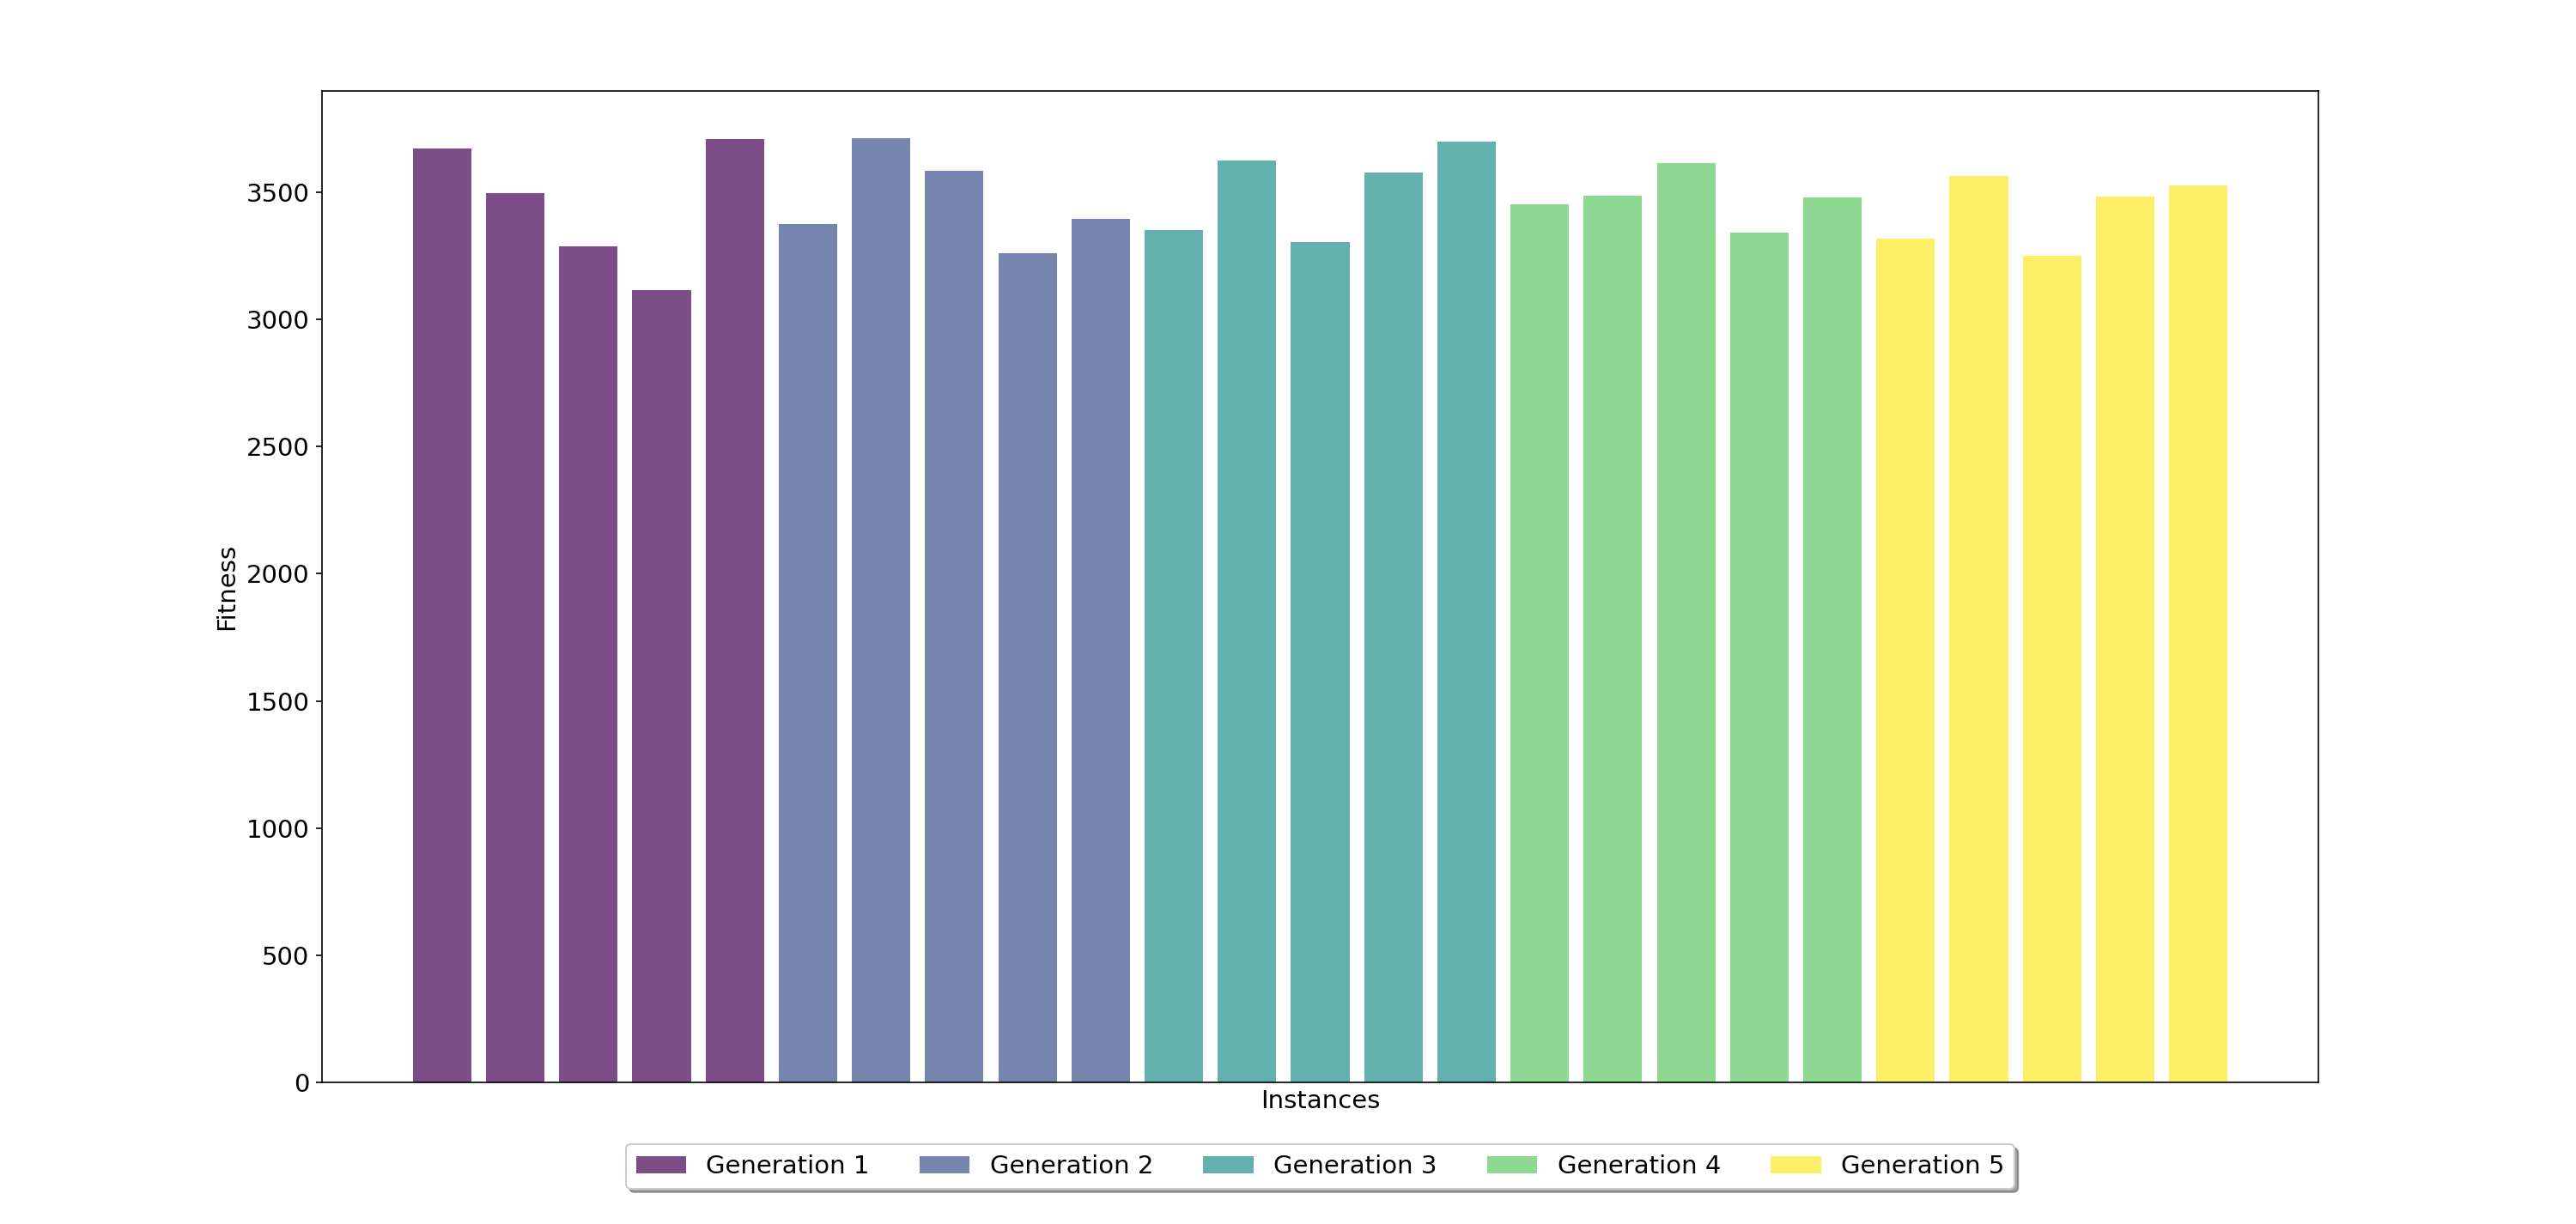
\includegraphics[width=\textwidth]{fig/14.png}
	\end{subfigure}
	\caption{贪婪协同进化算法最优各代的适应度值}
\end{figure}

\vspace{-12pt}

\begin{figure}[htbp]
	\centering
	\begin{subfigure}[b]{0.316\textwidth}
		\centering
		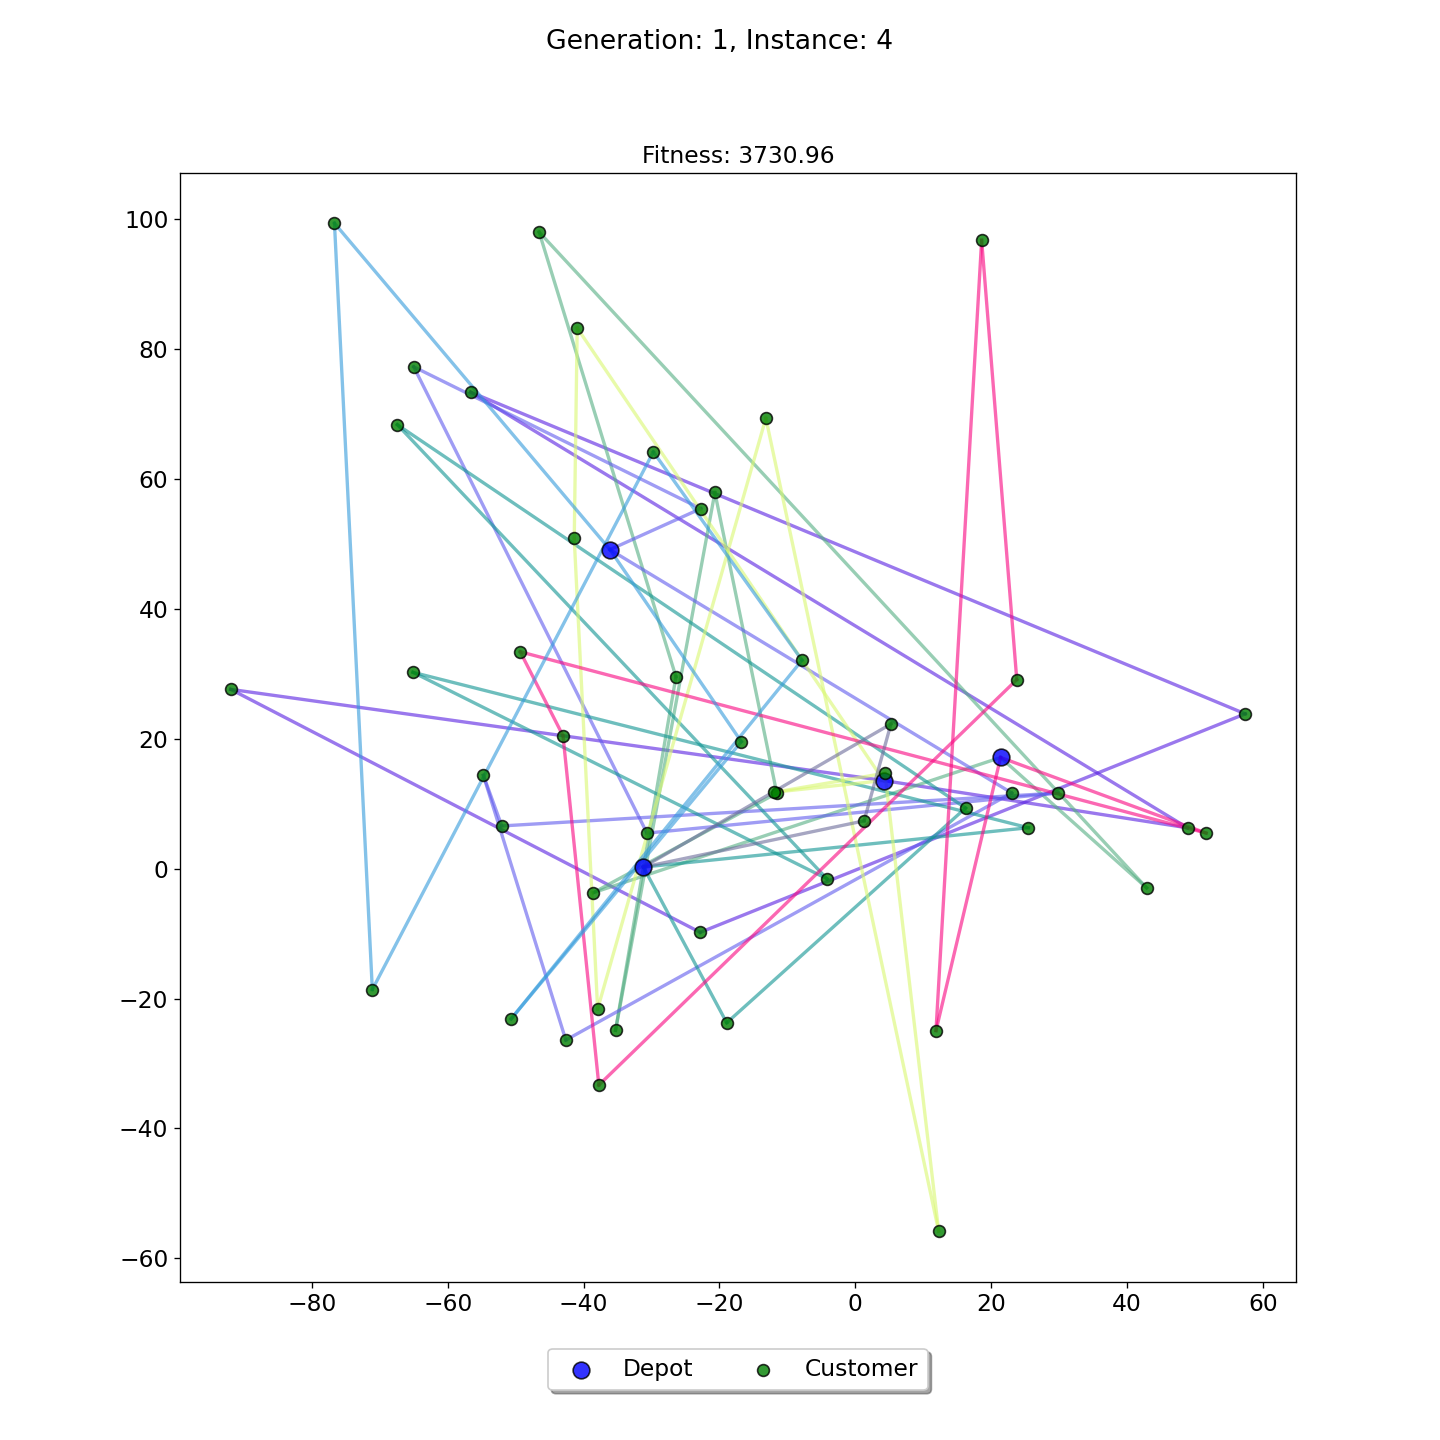
\includegraphics[width=\textwidth]{fig/15.png}
	\end{subfigure}
	\hspace{2pt} % Reduce horizontal space between images
	\begin{subfigure}[b]{0.4\textwidth}
		\centering
		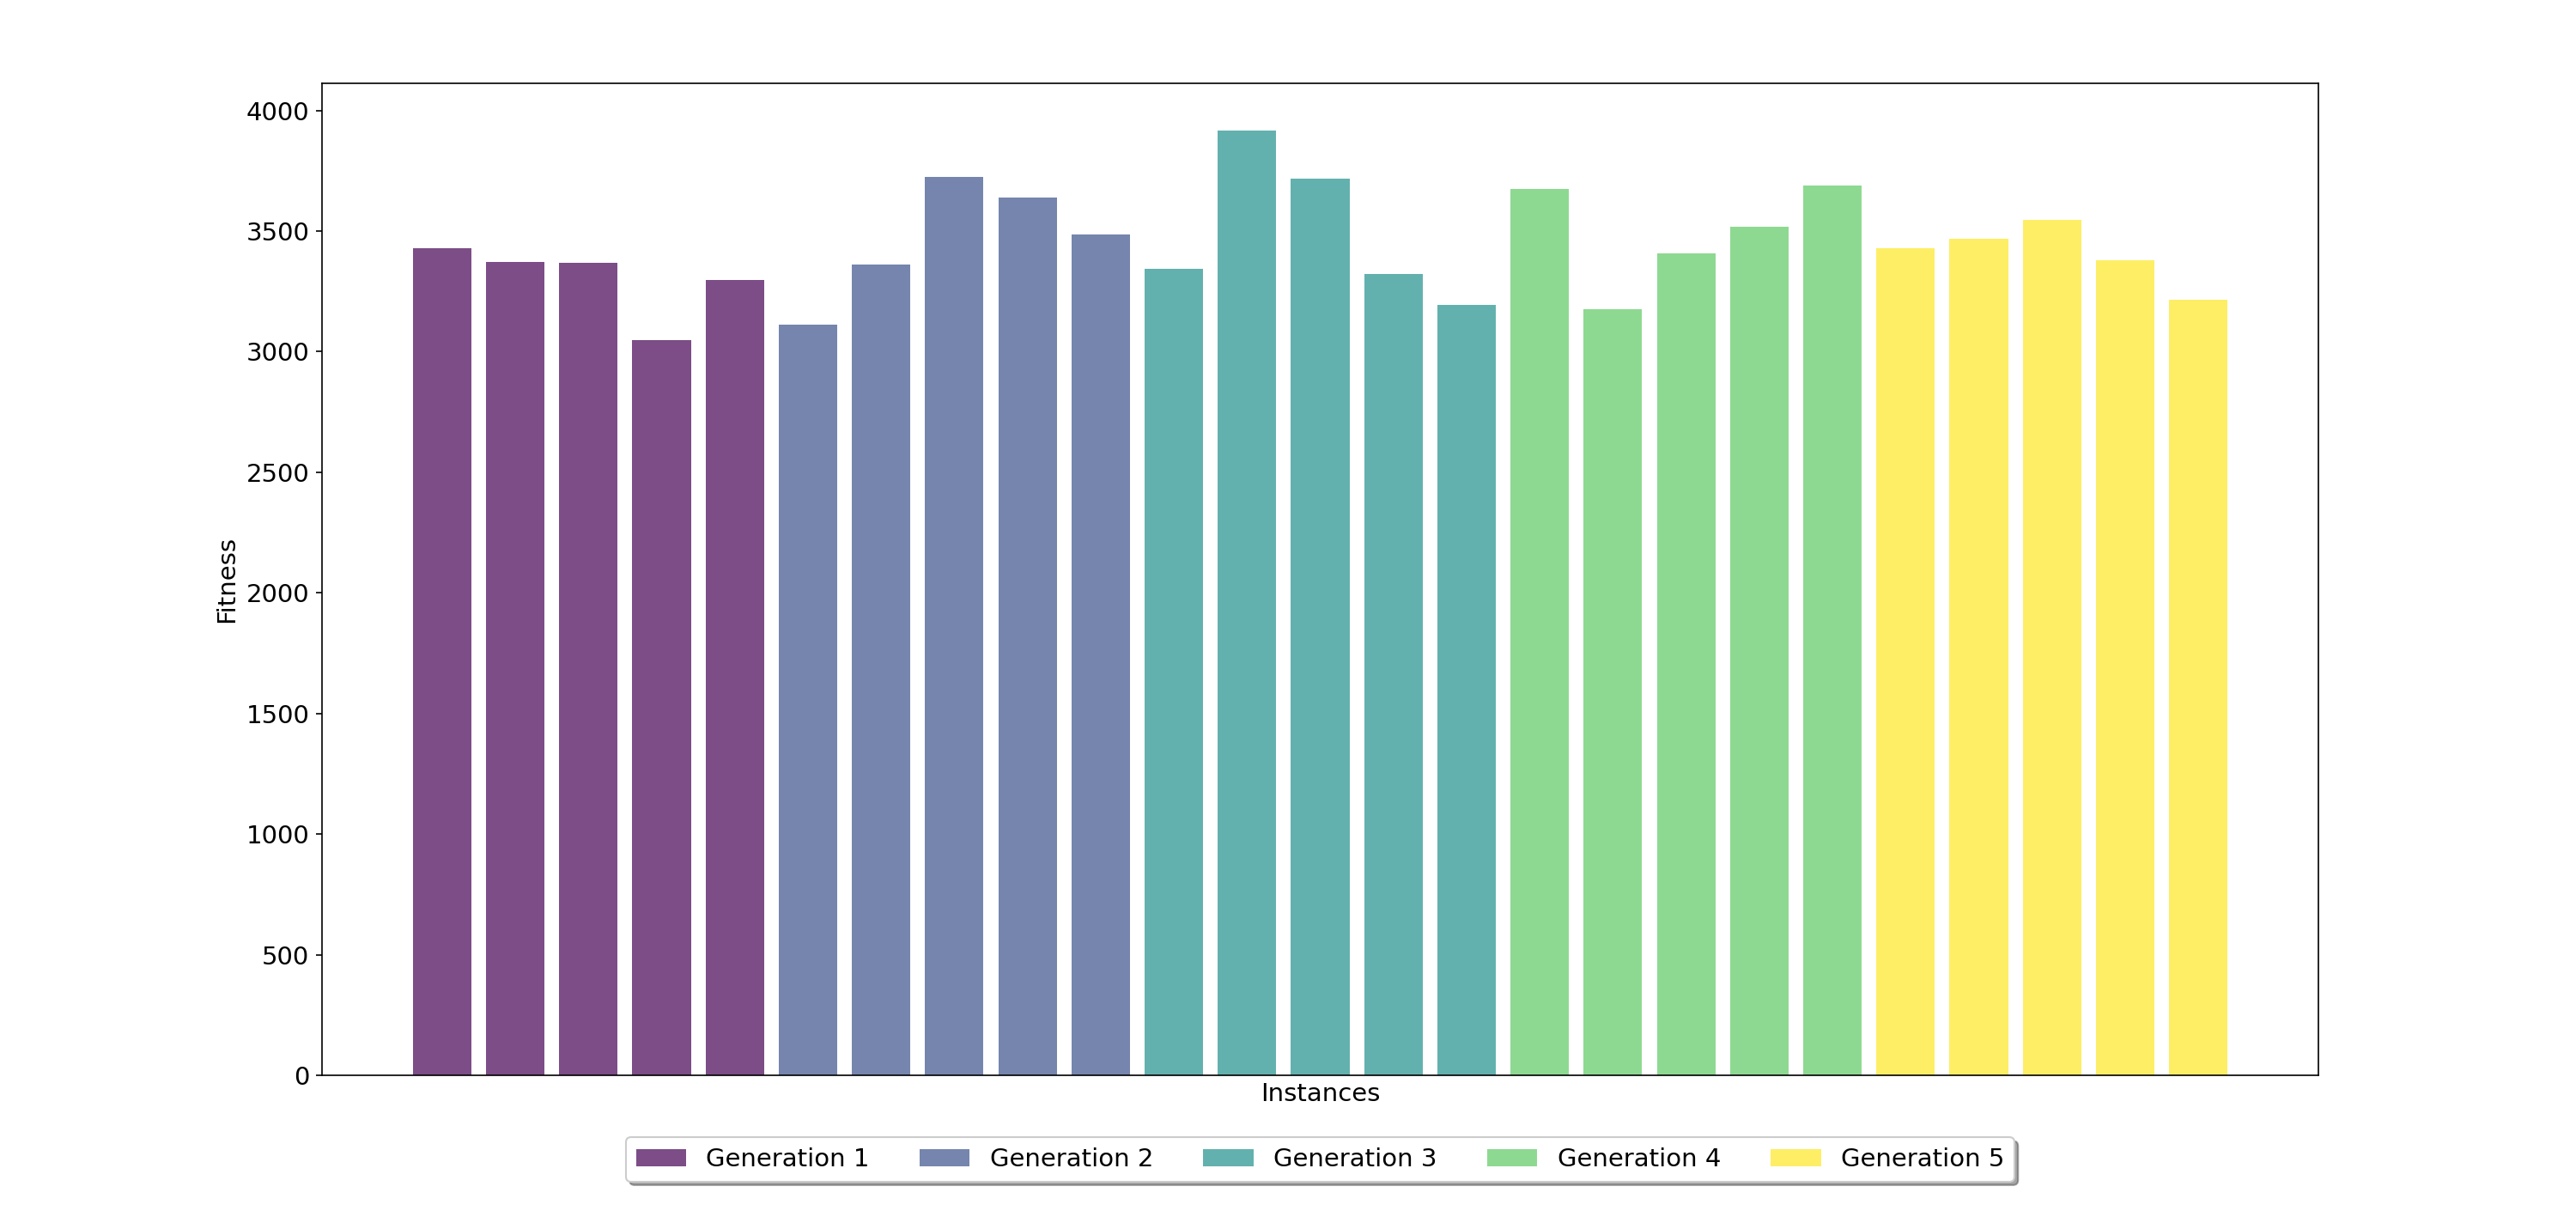
\includegraphics[width=\textwidth]{fig/16.png}
	\end{subfigure}
	\caption{禁忌搜索优化的贪婪协同进化算法最优各代的适应度值}
\end{figure}


	\newpage\
	\begin{table}[h!]
		\centering
		\caption{数据集 1 的性能比较}
		\begin{tabular}{lcccc}
			\toprule
			\textbf{算法} & \textbf{平均最终适应度} & \textbf{平均运行时间 (秒)} & \textbf{最佳最终适应度} \\
			\midrule
			EA    & 747.53 & 113.19 & 723.45 \\
			GCEA  & 730.44 & 119.87 & 683.08 \\
			TGCEA & 728.96 & 122.44 & 634.18 \\
			\bottomrule
		\end{tabular}
	\end{table}
	
	\begin{table}[h!]
		\centering
		\caption{数据集 2 的性能比较}
		\begin{tabular}{lcccc}
			\toprule
			\textbf{算法} & \textbf{平均最终适应度} & \textbf{平均运行时间 (秒)} & \textbf{最佳最终适应度} \\
			\midrule
			EA    & 3066.59 & 646.54 & 2983.45 \\
			GCEA  & 3052.84 & 669.87 & 2906.08 \\
			TGCEA & 3041.96 & 678.44 & 2873.18 \\
			\bottomrule
		\end{tabular}
	\end{table}

	
\subsection{讨论}

通过分析实验结果,我们可以得出以下关键结论:

首先,从适应度质量来看,贪婪协同进化算法(GCEA)和禁忌搜索优化的贪婪协同进化算法(TGCEA)在解的质量上均优于传统演化算法(EA)。在数据集1中,TGCEA的最佳适应度达到了634.18,显著优于GCEA的683.08和EA的723.45,显示了禁忌搜索策略在克服局部最优、提升解质量方面的有效性。在数据集2中,TGCEA的最佳适应度为2873.18,同样优于GCEA的2906.08和EA的2983.45,进一步证明了其在多样场景中的适应性。

其次,在计算效率方面,虽然TGCEA在解质量上更优,但其运行时间稍高,尤其是与EA相比。例如,在数据集1中,TGCEA的平均运行时间为122.44秒,EA则为113.19秒,这表明禁忌搜索引入了部分计算开销。然而,GCEA和TGCEA仍展现出良好的稳定性和效率平衡,说明协同进化算法能在保证高质量解的同时保持合理的计算效率。

最后,从鲁棒性和稳定性来看,TGCEA表现尤为突出。数据集2中的实验结果显示,TGCEA的平均适应度为3041.96,波动较小,而EA的平均适应度为3066.59,波动较大,说明TGCEA在不同的初始化条件下表现出更一致的解质量。相比之下,EA的适应度波动较大,显示出在不同实验条件下的稳定性较差。

\section{结论}

本研究通过比较演化算法(EA)、贪婪协同进化算法(GCEA)和禁忌搜索优化的贪婪协同进化算法(TGCEA)在多仓库车辆路径问题(MDVRP)中的表现,发现协同进化算法在解质量和稳定性上显著优于传统演化算法。GCEA通过协同进化策略提升了搜索效率,而TGCEA进一步结合禁忌搜索策略,在路径总距离和解质量上均取得了更好的结果。实验结果表明,协同进化方法在解决复杂优化问题方面具有较好的应用潜力,尤其在平衡计算时间与解质量的场景中,GCEA和TGCEA是更为优选的算法。
	
\newpage
\bibliographystyle{plain}
\bibliography{references}
	
	\newpage
	\begin{appendices}
	\section{算法评估图}
	\begin{figure}[h!]
		\centering
		\begin{subfigure}{0.32\textwidth}
			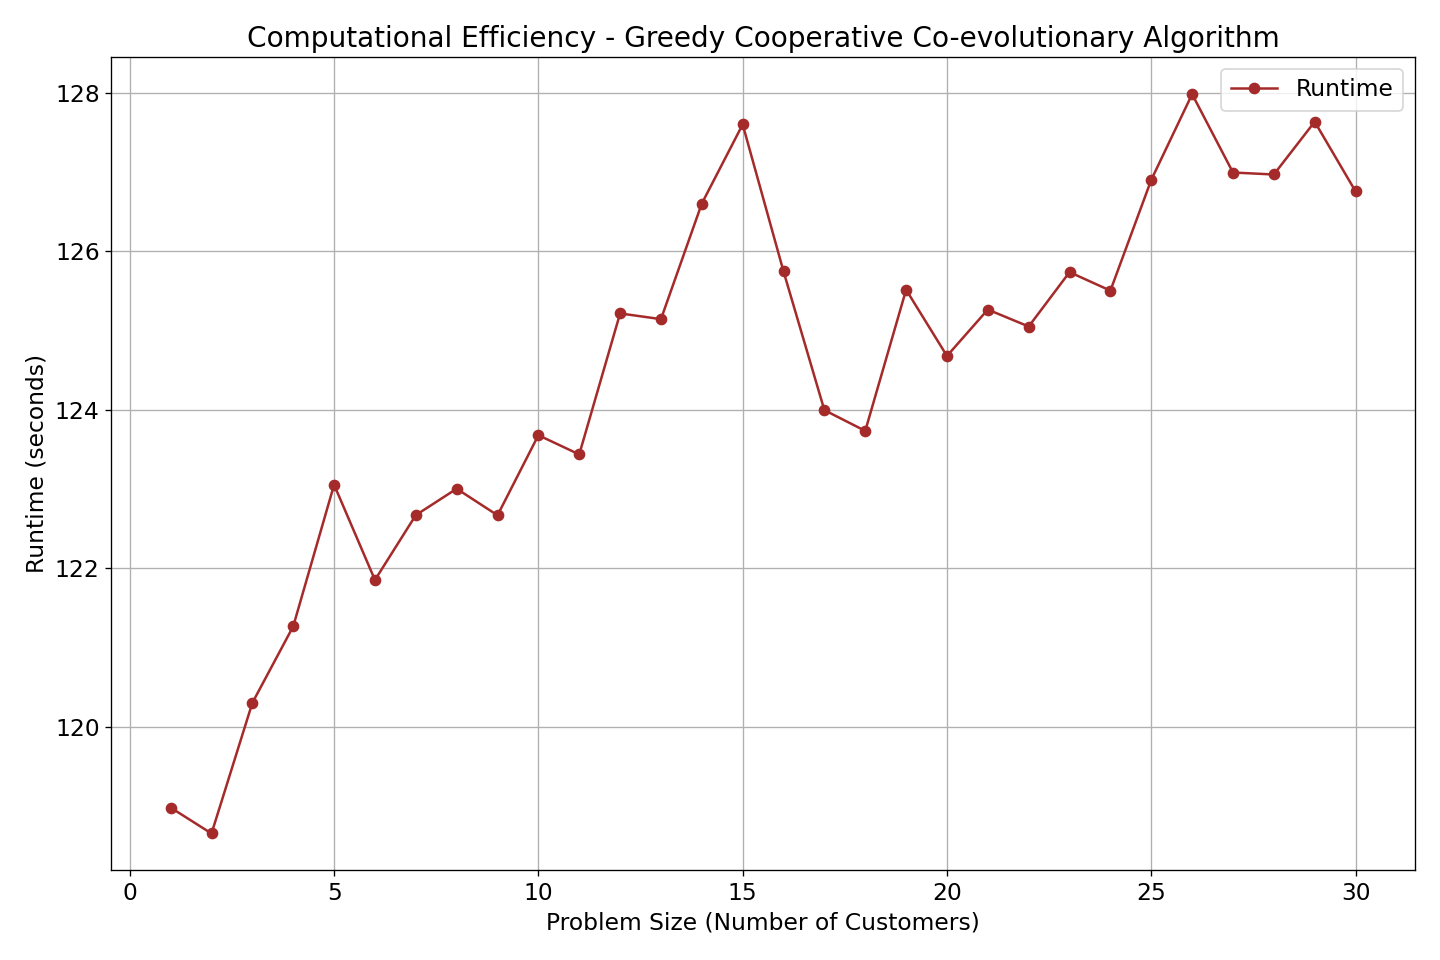
\includegraphics[width=\textwidth]{fig/22.png}
			\caption{GCEA 算法}
		\end{subfigure}
		\begin{subfigure}{0.32\textwidth}
			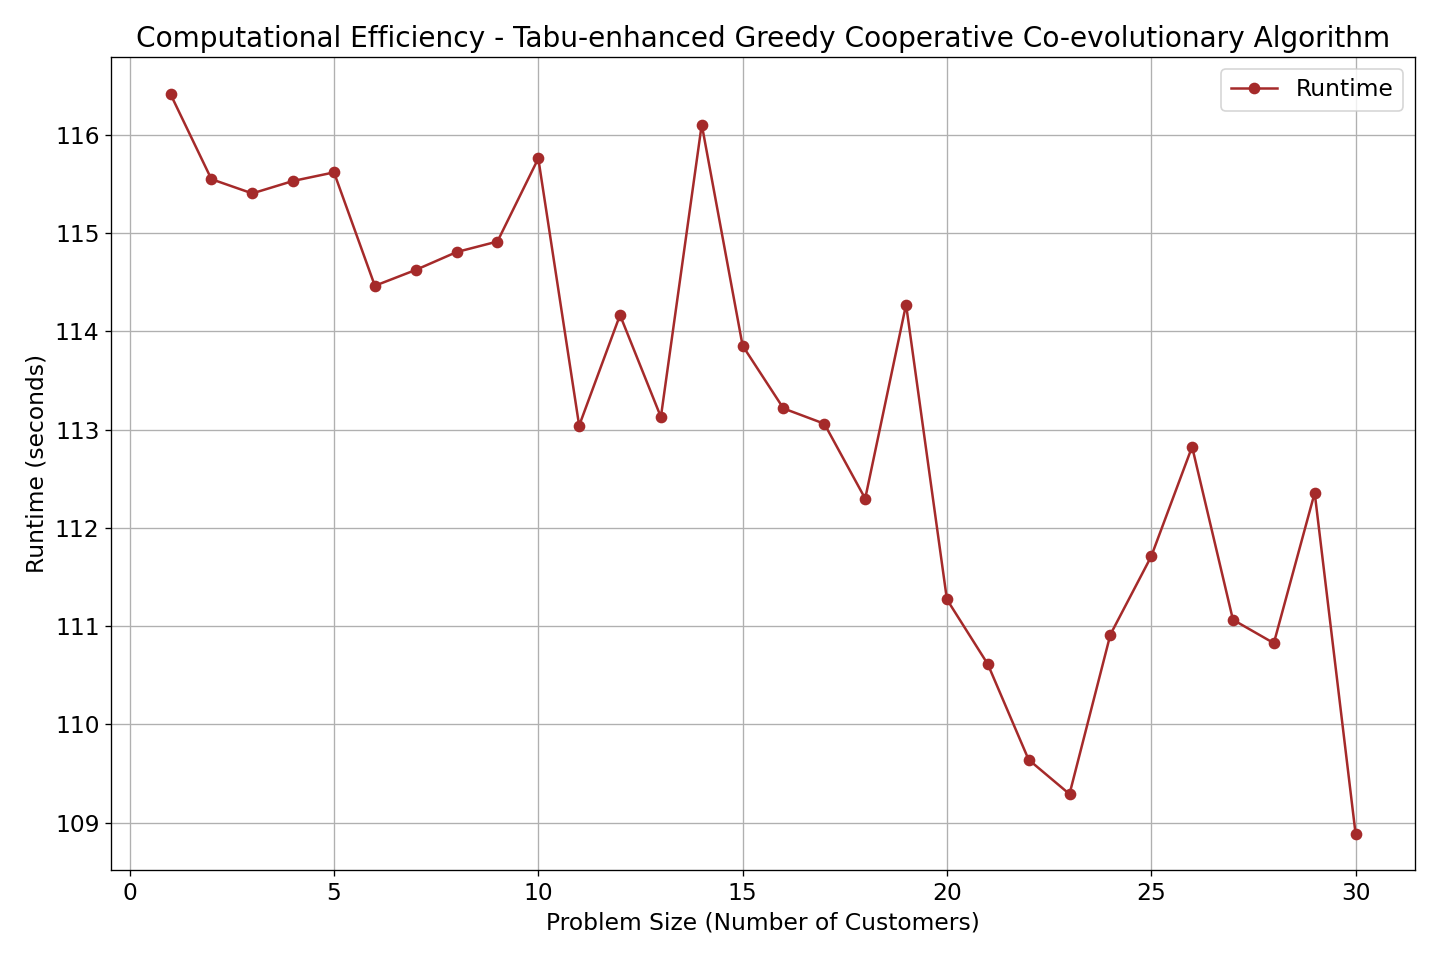
\includegraphics[width=\textwidth]{fig/27.png}
			\caption{TGCEA 算法}
		\end{subfigure}
		\begin{subfigure}{0.32\textwidth}
			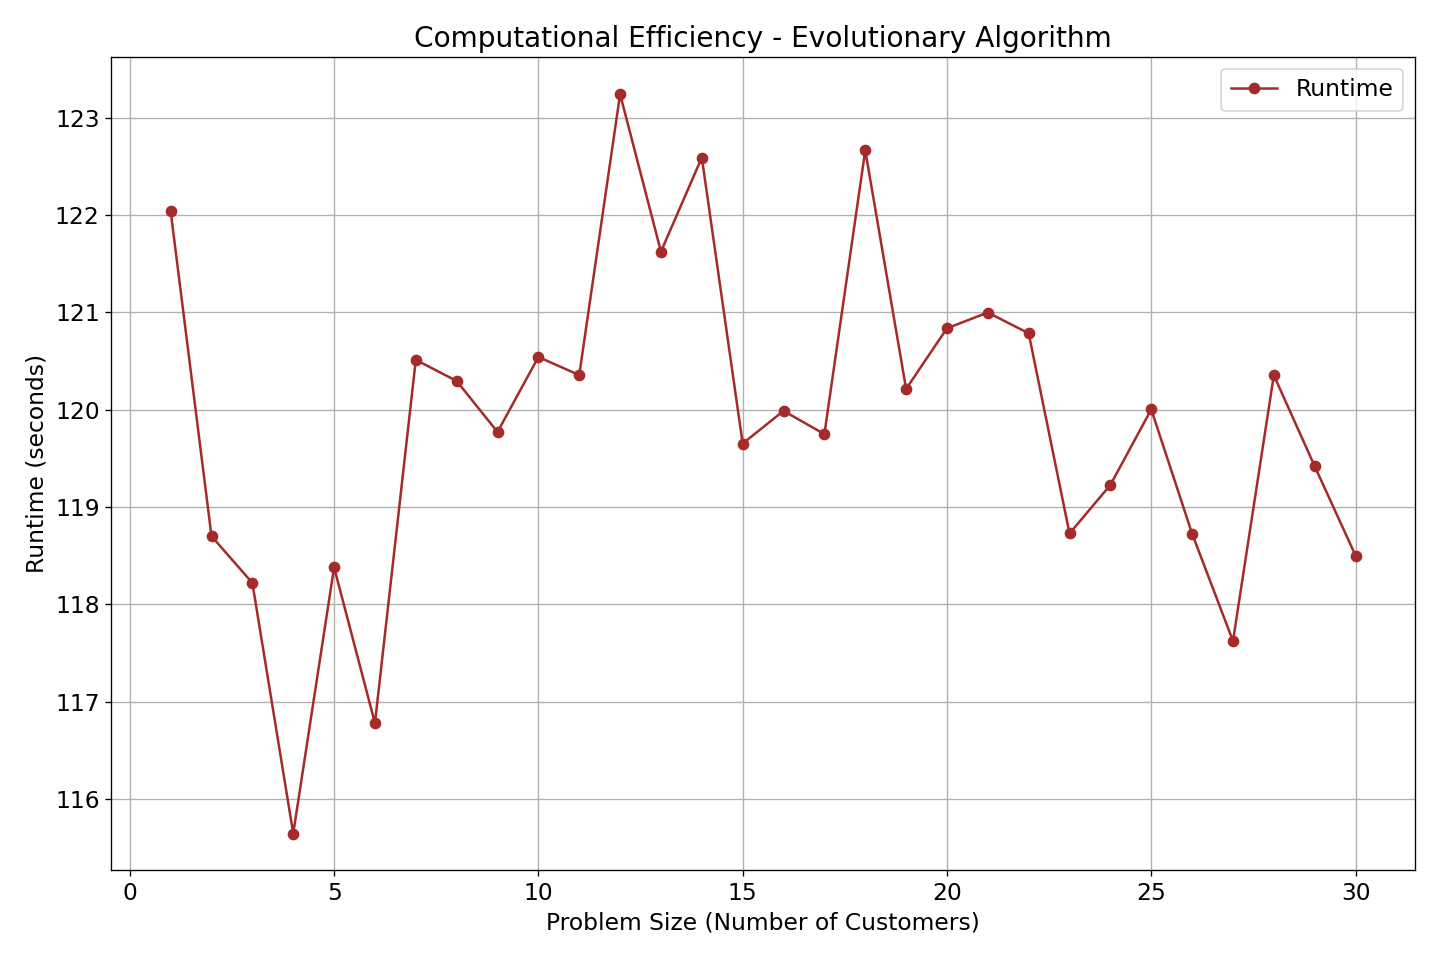
\includegraphics[width=\textwidth]{fig/18.png}
			\caption{EA 算法}
		\end{subfigure}
		\caption{数据集 1 的计算效率比较}
		\label{fig:dataset1_efficiency}
	\end{figure}
	
	\begin{figure}[h!]
		\centering
		\begin{subfigure}{0.32\textwidth}
			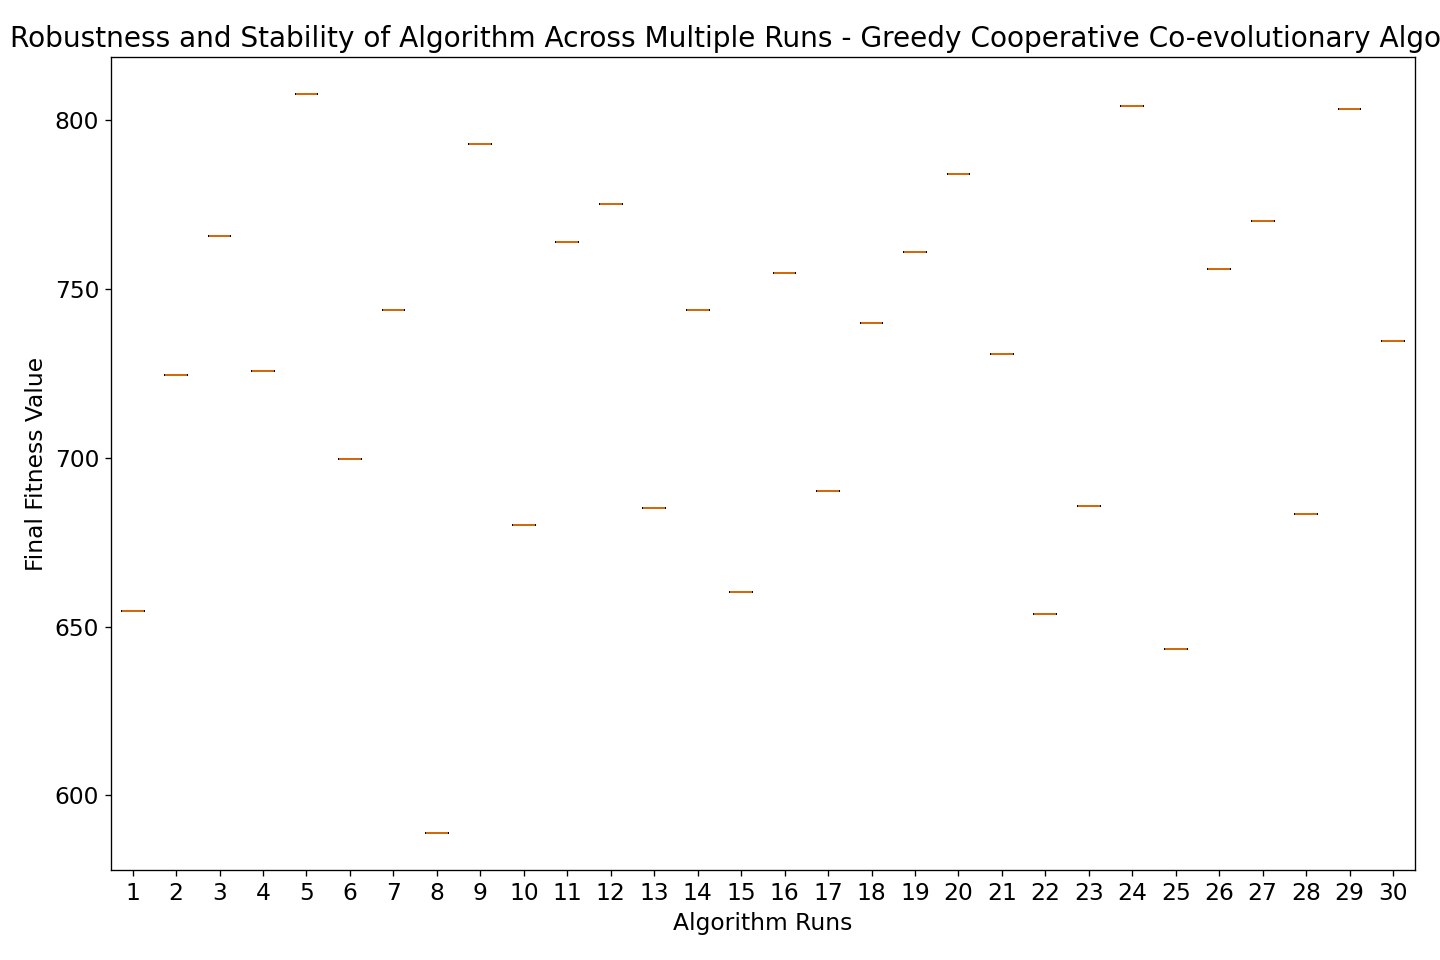
\includegraphics[width=\textwidth]{fig/23.png}
			\caption{GCEA 算法}
		\end{subfigure}
		\begin{subfigure}{0.32\textwidth}
			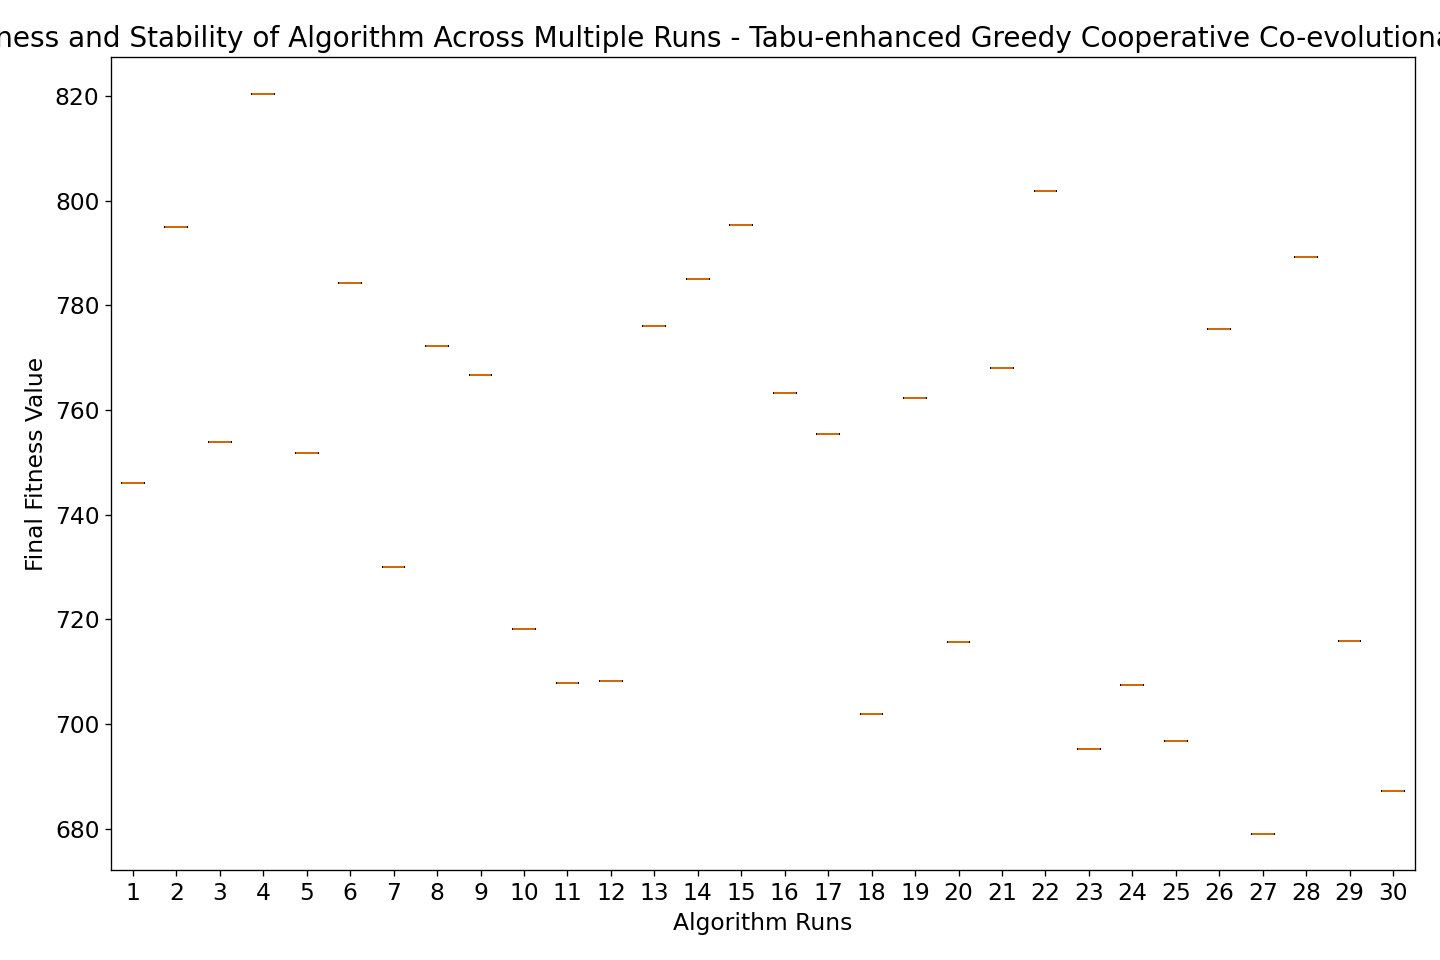
\includegraphics[width=\textwidth]{fig/25.png}
			\caption{TGCEA 算法}
		\end{subfigure}
		\begin{subfigure}{0.32\textwidth}
			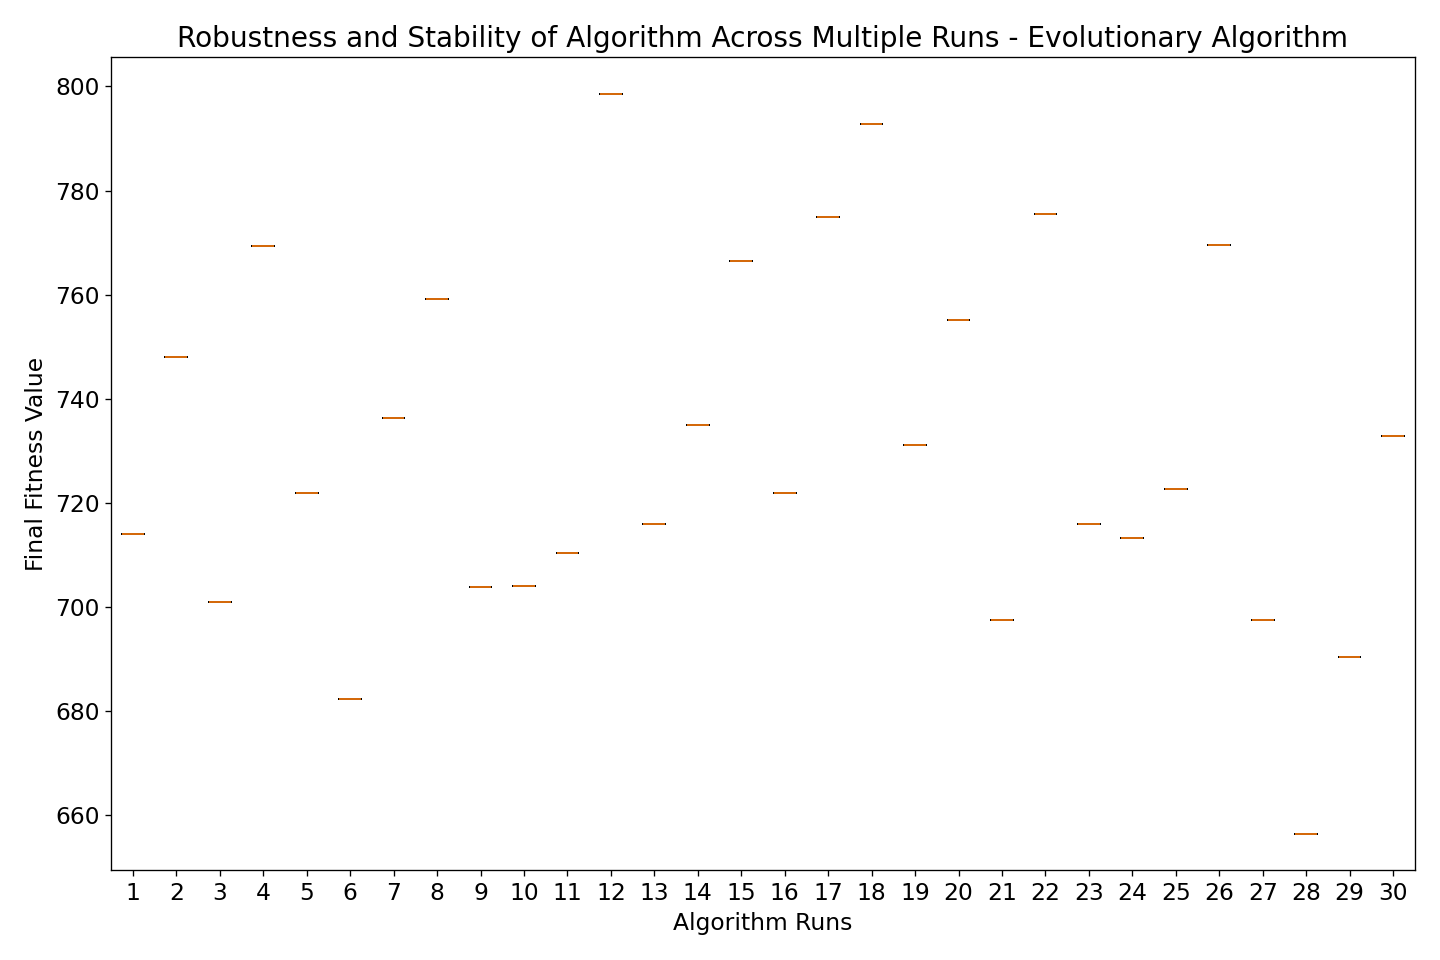
\includegraphics[width=\textwidth]{fig/20.png}
			\caption{EA 算法}
		\end{subfigure}
		\caption{数据集 1 的稳健性与稳定性比较}
		\label{fig:dataset1_stability}
	\end{figure}
	
	
	
	\begin{figure}[h!]
		\centering
		\begin{subfigure}{0.32\textwidth}
			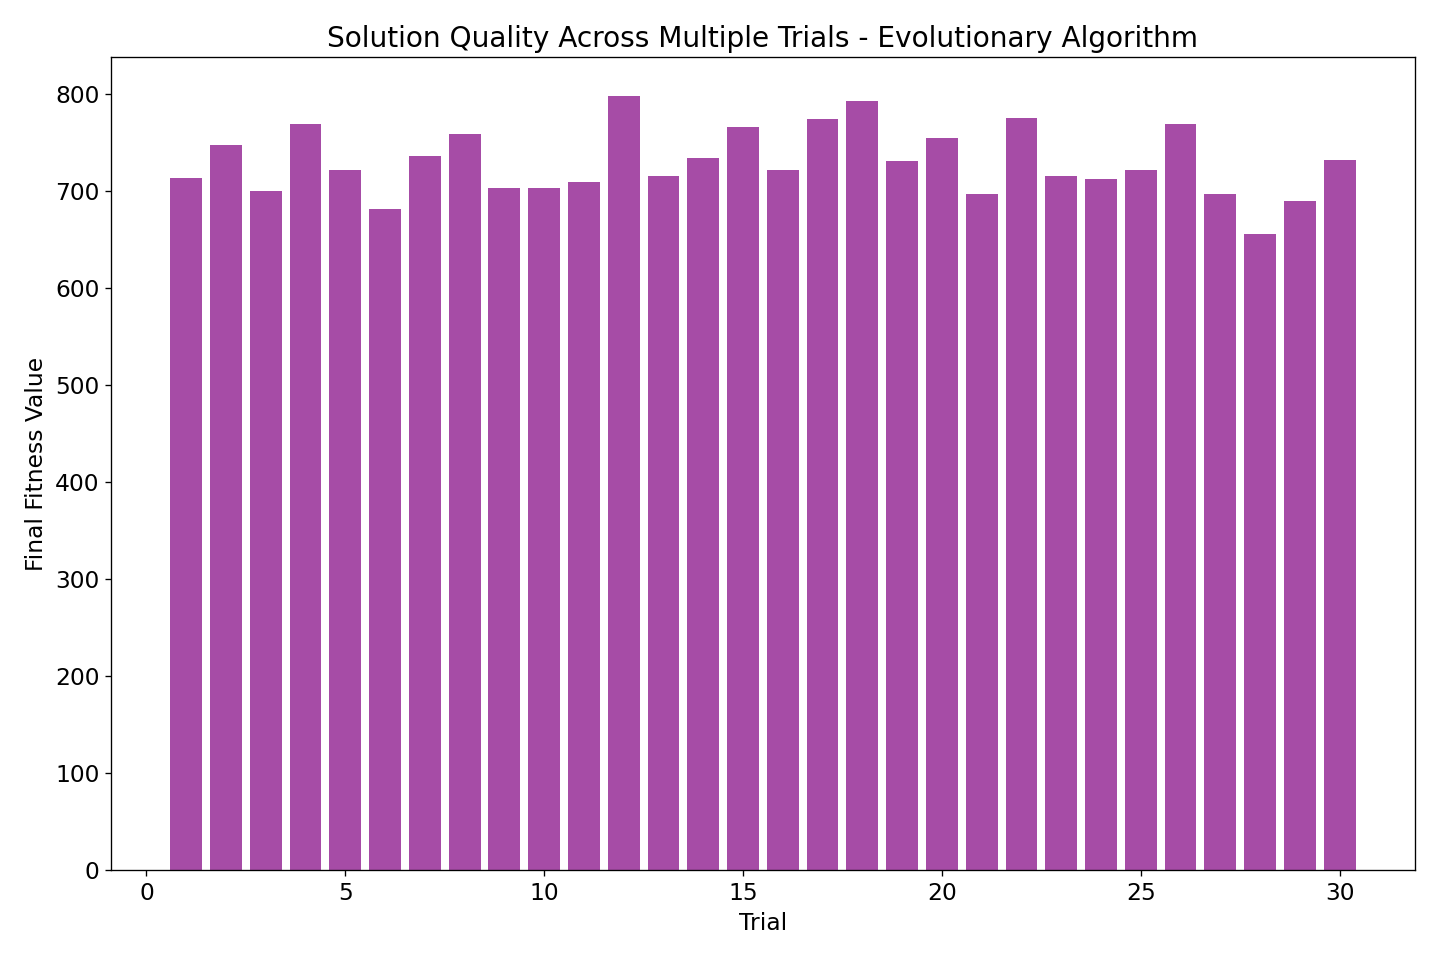
\includegraphics[width=\textwidth]{fig/17.png}
			\caption{EA 算法}
		\end{subfigure}
		\begin{subfigure}{0.32\textwidth}
			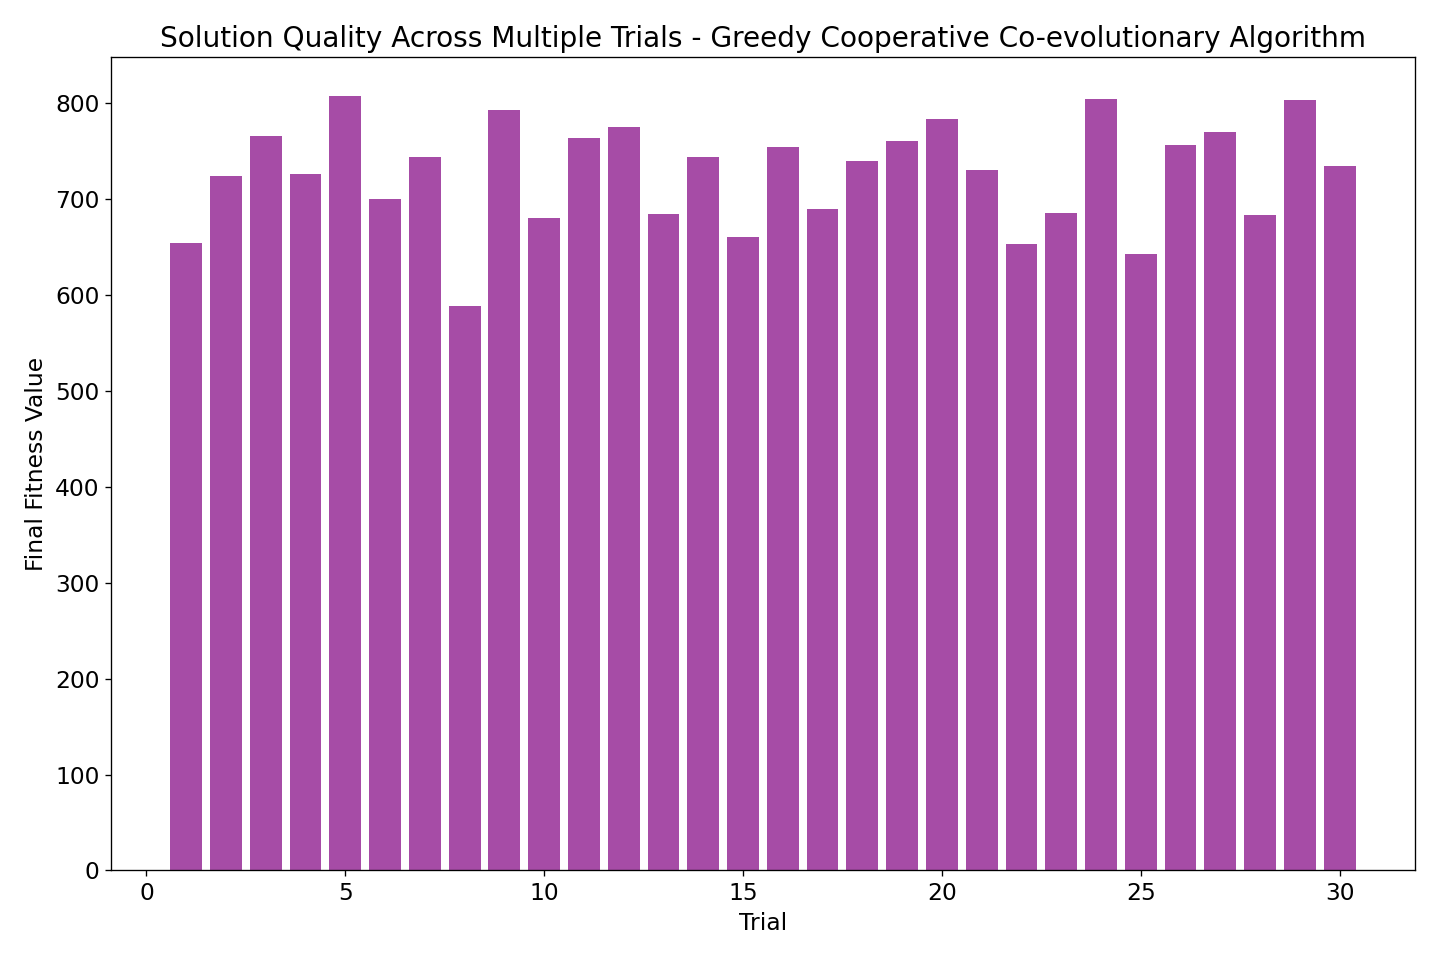
\includegraphics[width=\textwidth]{fig/24.png}
			\caption{GCEA 算法}
		\end{subfigure}
		\begin{subfigure}{0.32\textwidth}
			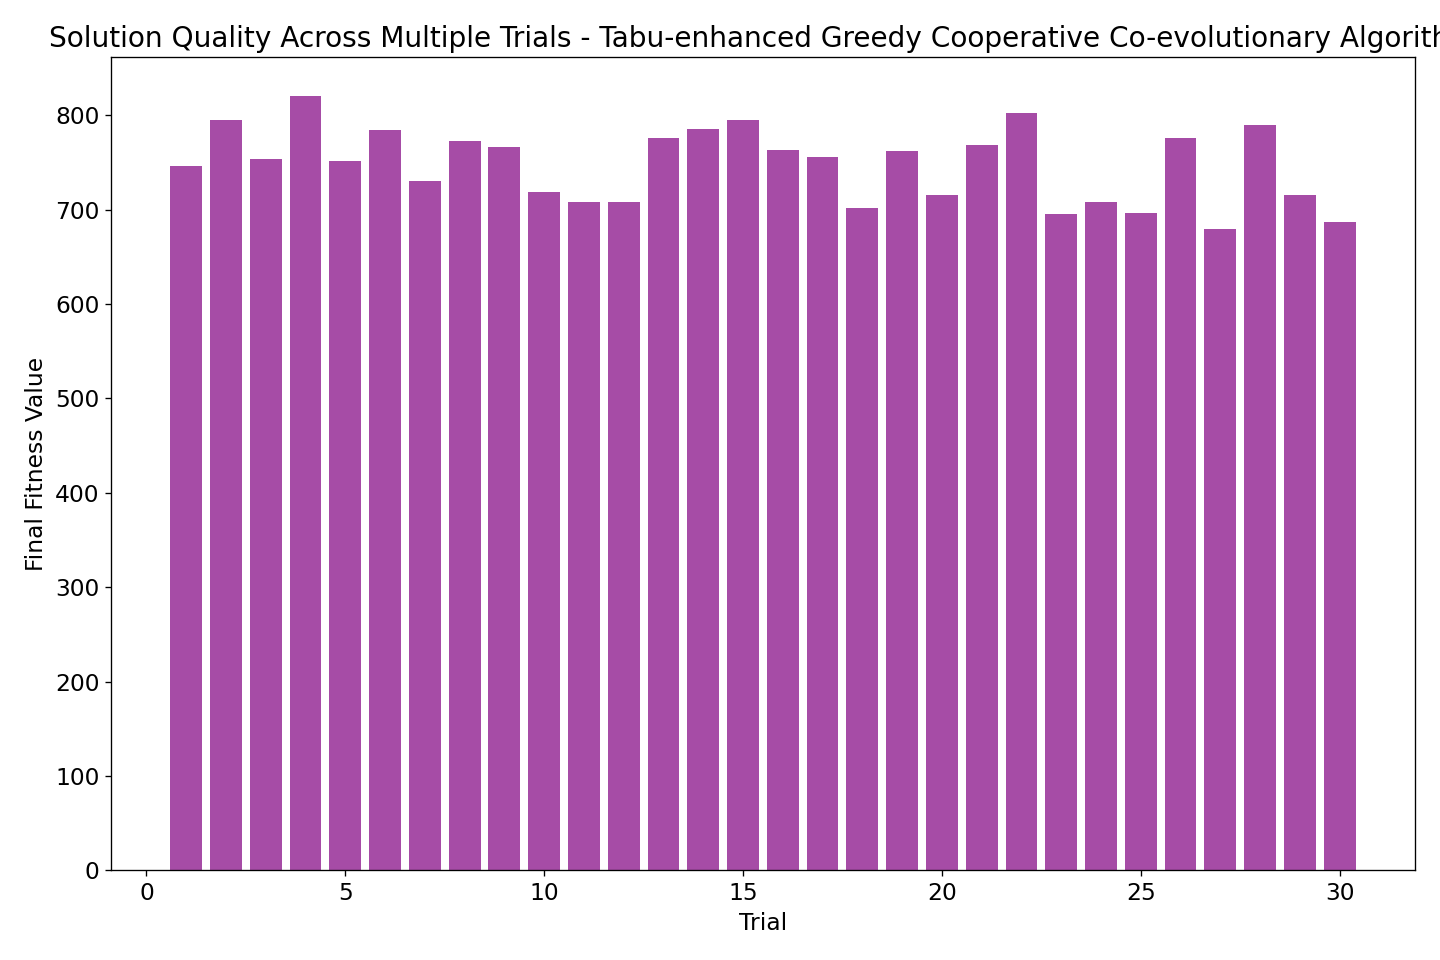
\includegraphics[width=\textwidth]{fig/26.png}
			\caption{TGCEA 算法}
		\end{subfigure}
		\caption{数据集 1 的多次求解质量比较}
		\label{fig:dataset1_solution_quality}
	\end{figure}



\end{appendices}	
\end{document}
